\ifdefined\maindoc\else
% typesetting this chapter as a standalone document
\def\doctitle{Contact and collisions}
% starting definitions for both the main document and stand-alone chapters
\documentclass{book}

\def\mech{artisynth.core.mechmodels}
\def\mgeo{maspack.geometry}

% Add search paths for input files
\makeatletter
\def\input@path{{../}{../../}{../texinputs/}}
\makeatother

\usepackage{amsmath}
\usepackage{framed}
%%
%% Default settings for artisynth
%%
\NeedsTeXFormat{LaTeX2e}
%%\ProvidesPackage{artisynthDoc}[2012/04/05]

\usepackage[T1]{fontenc}
\usepackage[latin1]{inputenc}
\usepackage{listings}
\usepackage{makeidx}
\usepackage{latexml}
\usepackage{graphicx}
\usepackage{framed}
\usepackage{booktabs}
\usepackage{color}

\newcommand{\pubdate}{\today}
\newcommand{\setpubdate}[1]{\renewcommand{\pubdate}{#1}}
\newcommand{\code}[1]{{\tt #1}}

\iflatexml
\usepackage{hyperref}
\setlength\parindent{0pt} 
\else
%% then we are making a PDF, so include things that LaTeXML can't handle: 
%% docbook style, \RaggedRight
\usepackage{ifxetex}
\usepackage{xstring}
\usepackage{pslatex} % fixes fonts; in particular sets a better-fitting \tt font

\usepackage[most]{tcolorbox}
\definecolor{shadecolor}{rgb}{0.95,0.95,0.95}
\tcbset{
    frame code={}
    center title,
    left=0pt,
    right=0pt,
    top=0pt,
    bottom=0pt,
    colback=shadecolor,
    colframe=white,
    width=\dimexpr\textwidth\relax,
    enlarge left by=0mm,
    boxsep=0pt,
    arc=0pt,outer arc=0pt,
}%

\usepackage[A4]{artisynth_papersize}
%\usepackage[letter]{artisynth_papersize}
\usepackage[hyperlink]{asciidoc-dblatex} 

%\usepackage{verbatim}
\usepackage{ragged2e}
\setlength{\RaggedRightRightskip}{0pt plus 4em}
\RaggedRight
\renewcommand{\DBKpubdate}{\pubdate}
\renewcommand{\DBKreleaseinfo}{}
\fi

% set hypertext links to be dark blue:
\definecolor{darkblue}{rgb}{0,0,0.8}
\definecolor{sidebar}{rgb}{0.5,0.5,0.7}
\hypersetup{colorlinks=true,urlcolor=darkblue,linkcolor=darkblue,breaklinks=true}

%%%%%%%%%%%%%%%%%%%%%%%%%%%%%%%%%%%%%%%%%%%%%%%%%%%%%%%%%%%%%%%%%%%%%%%%%%%%%
%
% Define macros for handling javadoc class and method references
%
%%%%%%%%%%%%%%%%%%%%%%%%%%%%%%%%%%%%%%%%%%%%%%%%%%%%%%%%%%%%%%%%%%%%%%%%%%%%%
\makeatletter

% macro to enable line break if inside a PDF file
\def\pdfbreak{\iflatexml\else\\\fi}

% code inspired by http://stackoverflow.com/questions/2457780/latex-apply-an-operation-to-every-character-in-a-string
\def\removeargs #1{\doremoveargs#1$\wholeString\unskip}
\def\doremoveargs#1#2\wholeString{\if#1$%
\else\if#1({()}\else{#1}\taketherest#2\fi\fi}
\def\taketherest#1\fi
{\fi \doremoveargs#1\wholeString}

% Note: still doesn't work properly when called on macro output ...
% i.e., \dottoslash{\concatnames{model}{base}{foo}} fails 
\def\dottoslash #1{\dodottoslash#1$\wholeString\unskip}
\def\dodottoslash#1#2\wholeString{\if#1$%
\else\if#1.{/}\else{#1}\fi\dottaketherest#2\fi}
\def\dottaketherest#1\fi{\fi \dodottoslash#1\wholeString}

\def\hashtodot #1{\dohashtodot#1$\wholeString\unskip}
\def\dohashtodot#1#2\wholeString{\if#1$X%
\else\if#1\#{.}\else{#1}\fi\hashtaketherest#2\fi}
\def\hashtaketherest#1\fi{\fi \dohashtodot#1\wholeString}

%\dollartodot{#1} does the same thing as \StrSubstitute[0]{#1}{\$}{.}
% from the packahe xstring. We define \dollartodot instead because
% LaTeXML does not implement xstring.
%
% Note that for the substituion to work, we need \ifx instead of \if,
% since otherwise escaped characters won't work properly:
% if #1 = \$, then \if#1* seems to compare '\' and '$' (and output '*'),
% rather than comparing '$' to '*'
\def\dollartodot #1{\dodollartodot#1*\wholeString\unskip}
\def\dodollartodot#1#2\wholeString{\ifx#1*%
\else \ifx#1\${.}\else{#1}\fi\dollartaketherest#2\fi}
\def\dollartaketherest#1\fi{\fi \dodollartodot#1\wholeString}

% concatenates up to three class/method names together, adding '.' characters
% between them. The first and/or second argument may be empty, in which case
% the '.' is omitted. To check to see if these arguments are empty, we
% use a contruction '\if#1@@', which will return true iff #1 is empty
% (on the assumption that #1 will not contain a '@' character).
\def\concatnames
#1#2#3{\if#1@@\if#2@@#3\else #2.#3\fi\else\if#2@@#1.#3\else#1.#2.#3\fi\fi}

\newcommand{\javabase}{}
\newcommand{\setjavabase}[1]{\renewcommand{\javabase}{#1}}

\def\artisynthDocBase{@ARTISYNTHDOCBASE}

\iflatexml
\def\ifempty#1{\def\temp{#1}\ifx\temp\empty}%
\newcommand{\artisynthManual}[3][]{%
   \ifempty{#1}
      \href{@ARTISYNTHDOCBASE/#2/#2.html}{#3}%
    \else
      \href{@ARTISYNTHDOCBASE/#1/#2.html}{#3}%
    \fi
}
\else
\newcommand{\artisynthManual}[3][]{%
\href{https://www.artisynth.org/@ARTISYNTHDOCBASE/#2.pdf}{#3}}
\fi

%\href{@ARTISYNTHDOCBASE/#2/#2.html}{#3}}



\newcommand{\javaclassx}[2][]{%
% Includes code to prevent an extra '.' at the front if #1 is empty. It
% works like this: if '#1' is empty, then '#1.' expands to '.', and so 
% '\if#1..' will return true, in which case we just output '#2'.
\href{@JDOCBEGIN/\concatnames{\javabase}{#1}{#2}@JDOCEND}{#2}}
\newcommand{\javaclass}[2][]{%
\href{@JDOCBEGIN/\concatnames{}{#1}{#2}@JDOCEND}{\dollartodot{#2}}}
\newcommand{\javaclassAlt}[2]{%
\href{@JDOCBEGIN/\concatnames{}{}{#1}@JDOCEND}{#2}}

\newcommand{\javamethodArgsx}[2][]{%
\href{@JDOCBEGIN/\concatnames{\javabase}{#1}{#2}@JDOCEND}{#2}}
\newcommand{\javamethodArgs}[2][]{%
\href{@JDOCBEGIN/\concatnames{}{#1}{#2}@JDOCEND}{#2}}
\newcommand{\javamethodAlt}[2]{%
\href{@JDOCBEGIN/\concatnames{}{}{#1}@JDOCEND}{#2}}
\newcommand{\javamethodAltx}[2]{%
\href{@JDOCBEGIN/\concatnames{\javabase}{}{#1}@JDOCEND}{#2}}

\newcommand{\javamethodNoArgsx}[2][]{%
\href{@JDOCBEGIN/\concatnames{\javabase}{#1}{#2}@JDOCEND}{\removeargs{#2}}}
\newcommand{\javamethodNoArgs}[2][]{%
\href{@JDOCBEGIN/\concatnames{}{#1}{#2}@JDOCEND}{\removeargs{#2}}}

\newcommand{\javamethod}{\@ifstar\javamethodNoArgs\javamethodArgs}
\newcommand{\javamethodx}{\@ifstar\javamethodNoArgsx\javamethodArgsx}

%%%%%%%%%%%%%%%%%%%%%%%%%%%%%%%%%%%%%%%%%%%%%%%%%%%%%%%%%%%%%%%%%%%%%%%%%%%%%
%
% Define macros for sidebars
%
%%%%%%%%%%%%%%%%%%%%%%%%%%%%%%%%%%%%%%%%%%%%%%%%%%%%%%%%%%%%%%%%%%%%%%%%%%%%%

\iflatexml
\newenvironment{sideblock}{\begin{quote}}{\end{quote}}
\else
\usepackage[strict]{changepage}
\definecolor{sidebarshade}{rgb}{1.0,0.97,0.8}
\newenvironment{sideblock}{%
    \def\FrameCommand{%
    \hspace{1pt}%
    {\color{sidebar}\vrule width 2pt}%
    %{\vrule width 2pt}%
    {\color{sidebarshade}\vrule width 4pt}%
    \colorbox{sidebarshade}%
  }%
  \MakeFramed{\advance\hsize-\width\FrameRestore}%
  \noindent\hspace{-4.55pt}% disable indenting first paragraph
  \begin{adjustwidth}{}{7pt}%
  %\vspace{2pt}\vspace{2pt}%
}
{%
  \vspace{2pt}\end{adjustwidth}\endMakeFramed%
}
\fi

\iflatexml
\newenvironment{shadedregion}{%
  \definecolor{shadecolor}{rgb}{0.96,0.96,0.98}%
  \begin{shaded*}%
% Put text inside a quote to create a surrounding blockquote that
% will properly accept the color and padding attributes
  \begin{quote}%
}
{%
  \end{quote}%
  \end{shaded*}%
}
\else
\newenvironment{shadedregion}{%
  \definecolor{shadecolor}{rgb}{0.96,0.96,0.98}%
  \begin{shaded*}%
}
{%
  \end{shaded*}%
}
\fi

% Wanted to create a 'listing' environment because lstlisting is
% tedious to type and because under latexml it may need
% some massaging to get it to work properly. But hard to do
% because of the verbatim nature of listing
%\iflatexml
%\newenvironment{listing}{\begin{lstlisting}}{\end{lstlisting}}%
%\else
%\newenvironment{listing}{\begin{lstlisting}}{\end{lstlisting}}%
%\fi

\iflatexml\else
% fancyhdr was complaining that it wanted a 36pt header height ...
\setlength{\headheight}{36pt}
\fi

% macro for backslash character
\newcommand\BKS{\textbackslash}

% macro for double hyphen (to prevent conversion of -- into -)
\newcommand\DHY{-{}-}

% Convenience stuff
\newcommand{\ifLaTeXMLelse}[2]{%
  \iflatexml %
  #1 %
  \else %
  #2 %
  \fi %
}

\newcommand{\ifLaTeXML}[1]{ %
  \iflatexml %
  #1 %
  \fi %
}

% new methodtable environment for documenting methods

% base width of the method table
\newlength{\methodtablewidth}
\iflatexml
\setlength{\methodtablewidth}{1.4\textwidth}
\else
\setlength{\methodtablewidth}{0.94\textwidth}
\fi
% horizontal space added at end of call to \methodentry
\newlength{\methodskip}
\setlength{\methodskip}{0pt}
% lengths set inside methodtable environment:
\newlength{\methodsiglength} % length of the method signature
\newlength{\methodcomlength} % length of the method comment
\setlength{\methodsiglength}{0.5\methodtablewidth}
\setlength{\methodcomlength}{0.5\methodtablewidth}

% command to add a method to a method table:
% arg #1: package and signature for finding URL
% arg #2: anchor text
% arg #3: comment describing the method
\newcommand{\methodentry}[3]{%
\javamethodAlt{#1}{\parbox[t]{\methodsiglength}{#2}}&
{\parbox[t]{\methodcomlength}{#3}}\\%
\noalign{\vspace{\methodskip}}}

% methodtable environment takes two arguments, both scale factors for
% methodtablewidth:
% arg #1: width of the method signature column
% arg #2: width of the method comment column
\newenvironment{methodtable}[3][0pt]{%
\begingroup
\setlength{\topskip}{0pt}
\setlength{\methodskip}{#1}
\setlength{\methodsiglength}{#2\methodtablewidth}%
\setlength{\methodcomlength}{#3\methodtablewidth}%
\iflatexml
\begin{snugshade}
\else
\begin{tcolorbox}
\fi
\renewcommand{\arraystretch}{1}
\begin{tabular}{ll}}{%
\end{tabular}
\renewcommand{\arraystretch}{1}
\iflatexml
\end{snugshade}
\else
\end{tcolorbox}
\fi
\endgroup}

% commands for added top, mid and bottom lines in the table.
% uses booktabs for PDF, regular hline for HTML
\newcommand{\topline}{\iflatexml\hline\else\toprule\fi}
\newcommand{\midline}{\iflatexml\hline\else\midrule\fi}
\newcommand{\botline}{\iflatexml\hline\else\bottomrule\fi}
\newcommand{\blankline}{%
\multicolumn{2}{l}{\iflatexml{@SPACE}\else\phantom{M}\fi}\\}%
% add vertical space within a two colum method environment
\newcommand{\methodspace}[1]{%
\iflatexml
\multicolumn{2}{l}{@VERTSPACE[#1]}\\
\else
\noalign{\vspace{#1}}%
\fi}%
% break a line and add an indentation of 1em
\newcommand{\brh}{\\\phantom{M}}

\makeatother

\def\matl{\left(\begin{matrix}}
\def\matr{\end{matrix}\right)}

\def\Bthe{\boldsymbol\theta}
\def\Btau{\boldsymbol\tau}
\def\Bom{\boldsymbol\omega}
\def\Bdel{\boldsymbol\delta}
\def\Blam{\boldsymbol\lambda}
\def\Bphi{\boldsymbol\phi}
\def\Bxi{\boldsymbol\xi}
\def\Bgam{\boldsymbol\gamma}
\def\Bsig{\boldsymbol\sigma}
\def\Bnu{\boldsymbol\nu}
\def\Bmu{\boldsymbol\mu}

\def\A{{\bf A}}
\def\B{{\bf B}}
\def\C{{\bf C}}
\def\D{{\bf D}}
\def\F{{\bf F}}
\def\G{{\bf G}}
\def\H{{\bf H}}
\def\I{{\bf I}}
\def\J{{\bf J}}
\def\K{{\bf K}}
\def\Jc{{\bf J}_c}
\def\L{{\bf L}}
\def\M{{\bf M}}
\def\N{{\bf N}}
\def\O{{\bf O}}
\def\P{{\bf P}}
\def\Q{{\bf Q}}
\def\R{{\bf R}}
\def\T{{\bf T}}
\def\U{{\bf U}}
\def\W{{\bf W}}
\def\X{{\bf X}}
\def\Minv{{\bf M}^{-1}}

\def\a{{\bf a}}
\def\b{{\bf b}}
\def\c{{\bf c}}
\def\d{{\bf d}}
\def\e{{\bf e}}
\def\f{{\bf f}}
\def\g{{\bf g}}
\def\k{{\bf k}}
\def\l{{\bf l}}
\def\m{{\bf m}}
\def\n{{\bf n}}
\def\p{{\bf p}}
\def\q{{\bf q}}
\def\r{{\bf r}}
\def\u{{\bf u}}
\def\v{{\bf v}}
\def\w{{\bf w}}
\def\x{{\bf x}}
\def\y{{\bf y}}
\def\z{{\bf z}}

\def\ma{{\bf m}_\alpha}
\def\mb{{\bf m}_\beta}
\def\va{{\bf v}_\alpha}
\def\vb{{\bf v}_\beta}
\def\vp{{\bf v}_\rho}
\def\vk{{\bf v}_k}
\def\ua{{\bf u}_\alpha}
\def\ub{{\bf u}_\beta}
\def\uk{{\bf u}_k}
\def\uj{{\bf u}_j}
\def\mar{{\bf m}_{\alpha r}}
\def\mbr{{\bf m}_{\beta r}}

\def\Maa{{\bf M}_{\alpha\alpha}}
\def\Mab{{\bf M}_{\alpha\beta}}
\def\Mba{{\bf M}_{\beta\alpha}}
\def\Mbb{{\bf M}_{\beta\beta}}
\def\hatMaa{\hat{\bf M}_{\alpha\alpha}}
\def\hatMab{\hat{\bf M}_{\alpha\beta}}
\def\hatMba{\hat{\bf M}_{\beta\alpha}}
\def\hatMbb{\hat{\bf M}_{\beta\beta}}
\def\Mbp{{\bf M}_{\beta\rho}}
\def\Map{{\bf M}_{\alpha\rho}}
\def\Mpa{{\bf M}_{\rho\alpha}}
\def\Mpb{{\bf M}_{\rho\beta}}
\def\Mpp{{\bf M}_{\rho\rho}}
\def\Mbk{{\bf M}_{\beta k}}
\def\Mak{{\bf M}_{\alpha k}}
\def\Mka{{\bf M}_{k\alpha}}
\def\Mkb{{\bf M}_{k\beta}}
\def\Mkk{{\bf M}_{kk}}

\def\Ga{{\bf G}_{\alpha}}
\def\Gp{{\bf G}_{\rho}}
\def\Gaa{{\bf G}_{\alpha\alpha}}
\def\Gab{{\bf G}_{\alpha\beta}}
\def\Gba{{\bf G}_{\beta\alpha}}
\def\Gbb{{\bf G}_{\beta\beta}}
\def\Gap{{\bf G}_{\alpha\rho}}
\def\Gpa{{\bf G}_{\rho\alpha}}
\def\Gbp{{\bf G}_{\beta\rho}}
\def\Gak{{\bf G}_{\alpha k}}
\def\Gka{{\bf G}_{k\alpha}}
\def\Gja{{\bf G}_{j\alpha}}
\def\Gkb{{\bf G}_{k\beta}}
\def\Gbk{{\bf G}_{\beta k}}

\def\lama{\Blam_{\alpha}}
\def\lamb{\Blam_{\beta}}
\def\lamp{\Blam_{\rho}}
\def\lamk{\Blam_{k}}
\def\lams{\Blam_{\sigma}}

\def\ba{{\bf b}_{\alpha}}
\def\bb{{\bf b}_{\beta}}
\def\fp{{\bf f}_{\rho}}
\def\fa{{\bf f}_{\alpha}}
\def\qa{{\bf q}_{\alpha}}
\def\qb{{\bf q}_{\beta}}
\def\za{{\bf z}_{\alpha}}
\def\zb{{\bf z}_{\beta}}
\def\wa{{\bf w}_{\alpha}}
\def\wb{{\bf w}_{\beta}}

\def\Na{\bar{\bf N}_{\alpha}}
\def\Nb{\bar{\bf N}_{\beta}}

\def\Up{{\bf U}_p}
\def\Un{{\bf U}_n}

\def\dFdl{\frac{\partial F}{\partial l}}
\def\dFddl{\frac{\partial F}{\partial \dot l}}

\def\Sr{s_\theta}
\def\Cr{c_\theta}
\def\Sp{s_\phi}
\def\Cp{c_\phi}
\def\Sy{s_\psi}
\def\Cy{c_\psi}
\def\Sa{s_{\alpha}}
\def\Ca{c_{\alpha}}
\def\Vp{v_{\phi}}


\iflatexml
\else
\usepackage{biblatex}
\addbibresource{references.bib}
\fi

\setcounter{tocdepth}{5}
\setcounter{secnumdepth}{3}

\title{\doctitle}
\ifdefined\maindoc
\author{John Lloyd and Antonio S\'anchez}
\setpubdate{Last update: March, 2022}

\iflatexml
\date{}
\fi
\fi

% graphics paths
\graphicspath{{./}{images/}}

% Listings settings
\definecolor{myblue}{rgb}{0,0,0.6}
\definecolor{mygreen}{rgb}{0,0.6,0}
\definecolor{mygray}{rgb}{0.5,0.5,0.5}
\definecolor{mylightgray}{rgb}{0.95,0.95,0.95}
\definecolor{mymauve}{rgb}{0.58,0,0.82}
\definecolor{myblack}{rgb}{0,0,0}
\lstset{
   language=Java,                   % text highlighting for Java
   breakatwhitespace=false,         % automatic breaks only at whitespace
   breaklines=true,                 % automatic line breaking
   commentstyle=\color{mygreen},    % comment style
   keepspaces=true,                 % keeps spaces in text
   keywordstyle=\color{myblue},     % keyword style
   numbers=none,                    % line-numbers; values: (none, left, right)
   numbersep=5pt,                   % how far the line-numbers are from code
   numberstyle=\tiny\color{mygray}, % line-numbers style
   showspaces=false,                % show spaces everywhere
   showstringspaces=false,          % underline spaces within strings
   showtabs=false,                  % show tabs
   stepnumber=1,                    % the step between two line-numbers
   stringstyle=\color{mymauve},     % string literal style
   tabsize=3,                       % sets default tabsize to 3 spaces
   backgroundcolor=\color{mylightgray}, % background color
   frame=single, 					% adds a frame around the code
   rulesepcolor=\color{mygray},
   rulecolor=\color{myblack},
   framerule=0pt,
   xleftmargin=2.2ex,               % numbers inside box
   framexleftmargin=2.2ex,			% indentation of frame
}

\begin{document}

\frontmatter

%\layout
\maketitle

\iflatexml{\large\pubdate}\fi

\tableofcontents

\mainmatter
% Scale latexml image sizes 2x
\newlength{\imglength}
\newcommand{\setlengthLaTeXML}[3]{ %
 \iflatexml %
 \setlength{#1}{#2} %
 \else %
 \setlength{#1}{#3} %
 \fi %
}
\fi


\chapter{Contact and Collision}
\label{ContactAndCollision:sec}

ArtiSynth supports contact and collisions between various collidable
bodies, including rigid bodies and FEM models, through a collision
handling mechanism build into {\tt MechModel}. Collisions are disabled
by default, but can be enabled between specific pairs of bodies, or
between general categories of {\it rigid} and {\it deformable} bodies
(Section \ref{EnablingCollisions:sec}). Collisions are supported
between any body that implements the interface
\javaclass[artisynth.core.mechmodels]{Collidable}.

Collision detection works by finding the intersecting regions between
the {\it collision meshes} of collidable bodies, and then using the
intersection information to determine contact points and their
associated constraints (Section \ref{CollisionImplementation:sec}).
Collision meshes must be instances of
\javaclass[maspack.geometry]{PolygonalMesh} and must be triangular;
mesh requirements are described in more detail in Section
\ref{CollisionMeshesAndCompounds:sec}. Typically, a collision mesh
is the same as the body's surface mesh, but other meshes (or
collections of meshes) can be specified instead
(Section \ref{CollisionMeshesAndCompounds:sec}).

Detailed aspects of the collision behavior, such as friction, optional
compliance and damping terms, methods used to determine contacts, and
various tolerances, can be controlled using
\javaclass[artisynth.core.mechmodels]{CollisionBehavior} objects
(Section \ref{ControllingCollisions:sec}). Collisions can be
visualized by rendering contact normals, forces, intersection
contours, and contact pressures (Section \ref{ContactRendering:sec}),
and information about specific collisions, including contact data,
forces, and pressures, can also be monitored as the simulation
proceeds (Section \ref{MonitoringCollisions:sec}).  

It is also possible to explicitly control contact forces by making
them an explicit function of penetration depth (Section
\ref{ContactRegularization:sec}); in particular, this capability is
used to support elastic foundation contact (Section
\ref{ElasticFoundationContact:sec}).

It should be understood that collision handling can be computationally
expensive and, due to its discontinuous nature, may be less accurate
than other aspects of the simulation.  ArtiSynth therefore provides a
number of ways to selectively control collision handling between
different pairs of bodies.  Collision handling is also challenging
because if collisions are enabled among $n$ objects, then one needs to
be able to easily specify the characteristics of up to $O(n^2)$
collision interactions, while also managing the fact that these
interactions are highly transient.  In ArtiSynth, collision handling
is managed by a
\javaclass[artisynth.core.mechmodels]{CollisionManager} that is a
subcomponent of each
\javaclass[artisynth.core.mechmodels]{MechModel}.  The collision
manager maintains default collision behaviors among certain groups of
collidable objects, while also allowing the user to override the
default behaviors by setting specific behaviors for any given pair of
collidables.

\begin{sideblock}
Within ArtiSynth, the terms collision and contact are used somewhat
interchangeably, although we acknowledge that in the literature,
collision is generally understood to refer to the transient process
that occurs when bodies first come into contact, while contact refers
to the more persistent situation as the bodies remain together.
\end{sideblock}

%\subsection{Collidable bodies}

\section{Enabling collisions}
\label{EnablingCollisions:sec}

\begin{sideblock}
This section describes how to enable collisions in code. However, it
is also possible to set some aspects of collision behavior using the
ArtiSynth GUI. See the section ``Collision handling'' in the
\artisynthManual{uiguide}{ArtiSynth User Interface Guide}.
\end{sideblock}

ArtiSynth can simulate collisions between bodies that implement the
interface \javaclass[artisynth.core.mechmodels]{Collidable}.
Collidable bodies are further subdivided into those that are {\it
rigid} and those that are {\it deformable}, according to whether their
\javamethod[artisynth.core.mechmodels.Collidable]{isDeformable()}
method returns {\tt true}. Rigid collidables include
\javaclass[artisynth.core.mechmodels]{RigidBody}, while deformable
collidables include FEM models 
(\javaclass[artisynth.core.femmodels]{FemModel3d}),
their mesh components
(\javaclass[artisynth.core.femmodels]{FemMeshComp}),
and skinned meshes 
(\javaclass[artisynth.core.femmodels]{SkinMeshBody},
Chapter \ref{skinning:sec}).
Because of the computational cost,
collision detection is turned off by default and must be explicitly
enabled when a model is built.  Collisions can be enabled between
specific pairs of bodies, or between general groupings of rigid and
deformable bodies.

Collision handling is implemented by a model's
\javaclass[artisynth.core.mechmodels]{MechModel}, which
contains a 
\javaclass[artisynth.core.mechmodels]{CollisionManager}
subcomponent that keeps track of which bodies are colliding and
computes the constraints and forces needed to enforce the collision
behaviors. The collision manager itself can accessed by the {\tt
MechModel} method
%
\begin{lstlisting}[]
  getCollisionManager()
\end{lstlisting}
%
and can be used to query and set various collision properties, as
described further below.

\subsection{Collisions between specific bodies}
\label{specificCollisions:sec}

As indicated above, collidable bodies are typically components such as
rigid bodies or FEM models. Given two collidable bodies {\tt
collidable0} and {\tt collidable1}, the simplest way to enable
collisions between them is with the {\tt MechModel} methods
%
\begin{lstlisting}[]
  setCollisionBehavior (collidable0, collidable1, enabled)
  setCollisionBehavior (collidable0, collidable1, enabled, mu)
\end{lstlisting}
%
The first method enables collisions {\it without} friction, while the
second enables collisions with friction as specified by {\tt mu},
which is the coefficient of Coulomb (or dry) friction.  The {\tt mu}
value is ignored if {\tt enabled} is {\tt false}. Specifying a {\tt
mu} value of 0 disables friction, and the friction coefficient can
also be left undefined by specifying a {\tt mu} value less than 0, in
which case the coefficient is inherited from the global friction value
accessed by the {\tt MechModel} methods
%
\begin{lstlisting}[]
  setFriction (mu)
  double getFriction()
\end{lstlisting}
%
More detailed control over collision behavior can be achieved
using the method
%
\begin{lstlisting}[]
  setCollisionBehavior (collidable0, collidable1, behavior)
\end{lstlisting}
%
where {\tt behavior} is a
\javaclass[artisynth.core.mechmodels]{CollisionBehavior} object
(Section\ref{CollisionBehavior:sec}) that specifies both {\it enabled}
and {\it mu}, along with other, more detailed collision properties
(see Section \ref{CollisionBehavior:sec}).

The {\tt setCollisionBehavior()} methods work by adding a {\tt
CollisionBehavior} object to the collision manager as a
subcomponent. With the method {\tt
setCollisionBehavior(collidable0,collidable1,behavior)}, the behavior
object is created and supplied by the application.  With the other
methods, the behavior object is created automatically and returned by
the method. Once a behavior has been specified, it can then be queried
using
%
\begin{lstlisting}[]
  CollisionBehavior getCollisionBehavior (collidable0, collidable1)
\end{lstlisting}
%
This method will return {\tt null} if no behavior for the pair in
question has been explicitly set using one of the
\pdfbreak
{\tt setCollisionBehavior()} methods.

\begin{sideblock}
One should normally avoid enabling collisions between bodies that are
otherwise connected, for example, adjacent bodies in a linkage
connected by joints, in order to avoid conflicts between
the connection and the collision behavior. If collision interaction is
required between {\it parts} of two connected bodies, this can be
achieved in various ways as described in Section
\ref{CollisionMeshesAndCompounds:sec}.
\end{sideblock}

\begin{sideblock}
Because behaviors are proper components, it is {\it not} permissible
to add them to the collision manager twice. Specifically, the
following will produce an error:
\begin{verbatim}
   CollisionBehavior behav = new CollisionBehavior();
   behav.setDrawIntersectionContours (true); 
   mech.setCollisionBehavior (col0, col1, behav);
   mech.setCollisionBehavior (col2, col3, behav); // ERROR
\end{verbatim}
However, if desired, a new behavior can be created from an existing
one:
\begin{verbatim}
   CollisionBehavior behav = new CollisionBehavior();
   behav.setDrawIntersectionContours (true); 
   mech.setCollisionBehavior (col0, col1, behav);
   behav = new CollisionBehavior(behav);
   mech.setCollisionBehavior (col2, col3, behav); // OK
\end{verbatim}
\end{sideblock}

\subsection{Default collisions between groups}

For convenience, it is also possible to specific default collision
behaviors between different {\it groups} of collidables.

The default collision behavior between {\it all} collidables can
be controlled using the {\tt MechModel} methods
%
\begin{lstlisting}[]
  setDefaultCollisionBehavior (enabled, mu)
  setDefaultCollisionBehavior (behavior)
\end{lstlisting}
%
where {\tt enabled}, {\tt mu} and {\tt behavior} act as described in
Section \ref{specificCollisions:sec}.

\begin{sideblock} 
Because of the possible computational expense of collision detection,
default collision behaviors should be used with care.
\end{sideblock} 

In addition, a default collision behavior can be set for generic
groups of collidables using the {\tt MechModel} methods
%
\begin{lstlisting}[]
  setDefaultCollisionBehavior (group0, group1, enabled, mu)
  setDefaultCollisionBehavior (group0, group1, behavior)
\end{lstlisting}
%
where {\tt group0} and {\tt group1} are static instances of
\javaclass[artisynth.core.mechmodels]{Collidable\$Group} that
represent the groups described in Table \ref{CollisionGroups:tab}.
The groups {\tt Collidable.Rigid} and {\tt Collidable.Deformable}
denote collidables that are rigid and deformable, respectively.  The
group {\tt Collidable.AllBodies} denotes both rigid and deformable
bodies, and {\tt Collidable.Self} is used to enable self-collision,
which is described in greater detail in Section
\ref{CompoundCollidablesAndSelf:sec}.

\begin{table}[h]
\begin{center}
\begin{tabular}{|ll|}
\hline
Collidable group & description \\
\hline
Collidable.Rigid & rigid collidables (e.g., rigid bodies) \\
Collidable.Deformable & deformable collidables (e.g, FEM models) \\
Collidable.AllBodies & rigid and deformable collidables \\
Collidable.Self & enables self-intersection
for compound deformable collidables\\
Collidable.All & rigid and deformable collidables and self-intersection\\
\hline
\end{tabular}
\end{center}
\caption{Collision group types.}
\label{CollisionGroups:tab}
\end{table}

A call to one of the {\tt setDefaultCollisionBehavior()} methods will
override the effects of previous calls. So for instance, the code
sequence
%
\begin{lstlisting}[]
  mech.setDefaultCollisionBehavior (true, 0);
  mech.setDefaultCollisionBehavior (
     Collidable.Deformable, Collidable.Rigid, false, 0);
  mech.setDefaultCollisionBehavior (true, 0.2);
\end{lstlisting}
%
will initially enable collisions between all bodies with a friction
coefficient of 0, then {\it disable} collisions between deformable and
rigid bodies, and finally re-enable collisions between all bodies with
a friction coefficient of 0.2.

The default collision behavior between any pair of collidable groups can
be queried using
%
\begin{lstlisting}[]
  CollisionBehavior getDefaultCollisionBehavior (group0, group1)
\end{lstlisting}
%
where {\tt group0} and {\tt group1} are restricted to the
primary groups {\tt Collidable.Rigid}, {\tt Collidable.Deformable},
and {\tt Collidabe.Self}, since individual behaviors are not
maintained for the composite groups {\tt Collidable.AllBodies} and {\tt
Collidable.All}.

Specific collision behaviors set using the {\tt
setCollisionBehavior()} methods of Section \ref{specificCollisions:sec}
will override any default collision settings. In addition, the second
argument {\tt collidable1} of these methods can describe either an
individual collidable, {\it or} one of the groups of Table
\ref{CollisionGroups:tab}. For example, the code fragment
\begin{lstlisting}[]
  MechModel mech;
  RigidBody bodA; 
  FemModel3d femB;

  ...

  mech.setCollisionBehavior (bodA, Collidable.Deformable, true, 0.1);
  mech.setCollisionBehavior (femB, Collidable.AllBodies, true, 0.0);
  mech.setCollisionBehavior (bodA, femB, false, 0.0);
\end{lstlisting}
will enable collisions between {\tt bodA} and all deformable
collidables (with friction 0.1), as well as {\tt femB} and all
deformable and rigid collidables (with friction 0.0), while
specifically {\tt disabling} collisions between {\tt bodA} and {\tt
femB}.

To determine the actual behavior controlling collisions between two
collidables (whether due to a default behavior or one specified using
{\tt setCollisionBehavior()}), 
one may use the method
%
\begin{lstlisting}[]
  getActingCollisionBehavior (collidable0, collidable1)
\end{lstlisting}
%
where {\tt collidable0} and {\tt collidable1} must both be specific
collidable components and cannot be a group (such as {\tt
Collidable.Rigid} or {\tt Collidable.All}).  If one of the collidables
is a {\it compound} collidable (Section
\ref{CompoundCollidablesAndSelf:sec}), or has a collidability setting (Section
\ref{collidability:sec}) that prevents collisions, there may be no
consistent acting behavior, in which case the method returns {\tt
null}.

Collision behaviors take priority over each other in the following
order:

\begin{enumerate}

\item Behaviors specified using {\tt setCollisionBehavior()} involving
two {\it specific} collidables.

\item Behaviors specified using {\tt setCollisionBehavior()} involving
one {\it specific} collidable and a {\it group} of collidables
(indicated by a {\tt Collidable.Group}), with later specifications
taking priority over earlier ones.

\item Default behaviors specified using {\tt setDefaultCollisionBehavior()}.

\end{enumerate}

A collision behavior specified with
{\tt setCollisionBehavior()} can later be removed
using 
%
\begin{lstlisting}[]
  clearCollisionBehavior (collidable0, collidable1)
\end{lstlisting}
%
and {\it all} such behaviors in a {\tt MechModel} can be removed with
%
\begin{lstlisting}[]
  clearCollisionBehaviors()
\end{lstlisting}
%
Note that this latter call does {\it not} remove default behaviors
specified with {\tt setDefaultCollisionBehavior()}.

\subsection{Example: collision with a plane}
\label{JointedCollide:sec}

A simple model illustrating collision between two jointed rigid bodies
and a plane is defined in
%
\begin{verbatim}
  artisynth.demos.tutorial.JointedCollide
\end{verbatim}
%

This model is simply a subclass of {\tt RigidBodyJoint} that
overrides the {\tt build()} method 
to add an inclined plane and enable collisions between it and
the two connected bodies:
%
\lstset{numbers=left}
\begin{lstlisting}[]
   public void build (String[] args) {

      super.build (args);

      bodyB.setDynamic (true);  // allow bodyB to fall freely

      // create and add the inclined plane
      RigidBody base = RigidBody.createBox ("base", 25, 25, 2, 0.2);
      base.setPose (new RigidTransform3d (5, 0, 0, 0, 1, 0, -Math.PI/8));
      base.setDynamic (false);
      mech.addRigidBody (base);

      // turn on collisions
      mech.setDefaultCollisionBehavior (true, 0.20);
      mech.setCollisionBehavior (bodyA, bodyB, false);
   }
\end{lstlisting}
\lstset{numbers=none}

The superclass {\tt build()} method called at line 3 creates
everything contained in {\tt RigidBodyJoint}. The remaining code then
alters that model: {\tt bodyB} is set to be dynamic (line 5) so that
it will fall freely, and an inclined plane is created from a thin box
that is translated and rotated and then set to be be non-dynamic
(lines 8-11).  Finally, collisions are enabled by setting the default
collision behavior (line 14), and then specifically disabling
collisions between {\tt bodyA} and {\tt bodyB} (line 15). As indicated
above, the latter step is necessary because the joint would otherwise
keep the two bodies in a permanent state of collision.

To run this example in ArtiSynth, select {\sf All demos > tutorial >
JointedCollide} from the {\sf Models} menu. The model should load and
initially appear as in Figure \ref{JointedCollide:fig}.  Running
the model (Section \ref{LoadingAndRunning:sec}) will
cause the jointed assembly to collide with and slide off the inclined
plane.

\begin{figure}[h]
\begin{center}
\iflatexml
 \includegraphics[]{images/JointedCollide}
\else
 \includegraphics[width=3.75in]{images/JointedCollide}
\fi
\end{center}
\caption{JointedCollide model loaded into ArtiSynth.}
\label{JointedCollide:fig}
\end{figure}

\subsection{Collisions for FEM models}
\label{sec:fem:collision}

Both \javaclass[artisynth.core.femmodels]{FemModel3d} and
\javaclass[artisynth.core.femmodels]{FemMeshComp} implement
\javaclass[artisynth.core.mechmodels]{Collidable}.  By default, a {\tt
FemModel3d} uses its surface mesh as the collision surface, while {\tt
FemMeshComp} will uses the mesh it contains (although collisions will
only occur if this is a triangular polygonal mesh).

Because {\tt FemModel3d} contains other collidables as subcomponents,
it is considered a {\tt compound} collidable, as discussed further in
Section \ref{CompoundCollidablesAndSelf:sec}. In particular, since
{\tt FemMeshComp} is also a {\tt Collidable}, we can enable collisions
with any embedded mesh inside an FEM.  Any forces resulting from the
collision are then automatically transferred back to the underlying
nodes of the model using Equation \eqref{pointFemForces:eqn}.

\begin{sideblock} {\bf Note:} Collisions involving shell elements are
not yet fully supported.  This relates to the fact that shells are
thin and can therefore pass through each other easily in a single time
step, and also that meshes associated with shell elements are usually
not closed.  However, collisions {\it should} work properly if

\begin{enumerate}

\item The collision meshes do not pass completely through each
other in a single time step;

\item Collisions do not occur near open mesh edges.

\end{enumerate}

Restriction 2 can often be relaxed if the collider type is set to {\tt
TRI\_INTERSECTION} (Section \ref{ColliderTypes:sec}).

\end{sideblock}

\subsection{Example: FEM models and rigid bodies}

\begin{figure}[ht]
	\centering
	\setlengthLaTeXML{\imglength}{0.8\textwidth}{0.6\textwidth}
	\includegraphics[width=\imglength]{images/FemCollisions}
	\caption{FemCollisions model loaded into ArtiSynth.}
	\label{fig:fem:collisions}
\end{figure}

An example of FEM collisions is shown in
Figure \ref{fig:fem:collisions}.  The full source code can be found in
the ArtiSynth repository under {\tt
artisynth.demos.tutorial.FemCollisions}. The model contains a rigid
body table and three FEM models: a beam (blue), an {\tt ellipsoid}
(red), and a hex block containing an embedded spherical mesh
(green).  The collision-enabling code is as follows:
\begin{lstlisting}[]
// Set up collisions
mech.setCollisionBehavior(ellipsoid, beam, true);   // beam-ellipsoid
mech.setCollisionBehavior(ellipsoid, table, true);  // ellipsoid-table
mech.setCollisionBehavior(table, beam, true);       // beam-table

FemMeshComp embeddedSphere = 
   block.getMeshComp("embedded");                   // get embedded FemMeshComp
mech.setCollisionBehavior(embeddedSphere, table, true);      // sphere-table
mech.setCollisionBehavior(ellipsoid, embeddedSphere, true);  // sphere-ellipsoid
\end{lstlisting}
This enables collisions between the ellipsoid and the beam, table and
embedded sphere, and between the table and the beam and embedded
sphere.  However, collisions are {\it not} enabled between the block
itself and any other components; notice in the figure that the block
surface passed through the table and ellipsoid.

\section{Collision behaviors and collidability}
\label{ControllingCollisions:sec}

\subsection{Collision behaviors}
\label{CollisionBehavior:sec}

As mentioned above,
\javaclass[artisynth.core.mechmodels]{CollisionBehavior} objects can
be used to control other aspects of contact beyond friction and
enabling. This may be done by setting the {\tt CollisionBehavior}
properties listed below. Except where otherwise indicated, these
properties are also exported by the collision manager, where they can
be used to provide global default settings for {\it all} collisions.

\begin{sideblock}
In addition to these properties, {\tt CollisionBehavior} and {\tt
CollisionManager} export other properties that can be used to control
the rendering of collisions, as described in
Section \ref{ContactRendering:sec}.
\end{sideblock}

\begin{description}

\item[enabled]\mbox{}

A boolean that determines if collisions are enabled. Not present
in the collision manager.

\item[friction]\mbox{}

A double giving the coefficient of Coulomb friction, typically in the
range $[0,0.5]$. The default value is 0. Setting friction to a
non-zero value increases the simulation time, since extra constraints
must be added to the system to accommodate the friction. 

\item[method]\mbox{}

An instance of
\javaclass[artisynth.core.mechmodels]{CollisionBehavior\$Method} that
controls how the contact constraints for the collision response are
generated. The methods, described in more detail in Section
\ref{ContactMethods:sec}, are:

\begin{tabular}{lll}
\hline
Method & Constraint generation \\
\hline
CONTOUR\_REGION & 
constraints generated from planes fit to each mesh contact region \\
VERTEX\_PENETRATION & constraints generated from penetrating vertices\\
VERTEX\_EDGE\_PENETRATION & 
constraints generated from penetrating vertices and edge-edge contacts\\
DEFAULT & method is determined automatically\\
INACTIVE & no constraints generated\\
\hline
\end{tabular}

The default value is {\tt DEFAULT}.

\item[vertexPenetrations]\mbox{}

An instance of
\javaclass[artisynth.core.mechmodels]{CollisionBehavior\$VertexPenetrations}
that controls the collidables for which vertex penetrations are
computed when using vertex penetration contact (see Sections
\ref{VertexPenetration:sec} and \ref{SettingContactMethod:sec}).
The default value is {\tt AUTO}.

\item[bilateralVertexContact]\mbox{}

A boolean which causes the system
to handle vertex penetration contact using bilateral constraints
instead of unilateral constraints.  This usually improves
computational performance significantly for collisions involving FEM
models, but may result in overconstrained contact when vertex penetration 
contact is used between rigid bodies, as well as in
some other circumstances (Section \ref{OverconstrainedContact:sec}).
The default value is {\tt true}.

\item[colliderType]\mbox{}

An instance of
\javaclass[artisynth.core.mechmodels]{CollisionManager\$ColliderType}
that specifies the underlying mechanism used to determine the
collision information between two meshes. The choice of collider may
restrict which collision {\it methods} (described above) are
allowed. Collider types are described in more detail in 
Section \ref{ContactMethods:sec} and include:

\begin{tabular}{lll}
\hline
Type & Description \\
\hline
AJL\_CONTOUR & uses mesh intersection contour to find penetrating 
regions and vertices\\
TRI\_INTERSECTION & uses triangle intersections to find penetrating 
regions and vertices \\
SIGNED\_DISTANCE & uses a signed distance field to find penetrating vertices\\
\hline
\end{tabular}

The default value is {\tt TRI\_INTERSECTION}.

\item[reduceConstraints]\mbox{}

A boolean which, if {\tt true}, indicates that the system should try
to reduce the number of contacts between bodies in order to try and
remove redundant contacts. See Section
\ref{OverconstrainedContact:sec}.  The default value is {\tt false}.

\item[compliance]\mbox{}

A double which adds a compliance (inverse stiffness) to the collision
behavior, so that the contact has a ``springiness''.  See Section
\ref{OverconstrainedContact:sec}. The default value for this is 0 (no
compliance).

\item[damping]\mbox{}

A double which, if {\sf compliance} is non-zero, specifies a damping
to accompany the compliant behavior. See Section
\ref{OverconstrainedContact:sec}.  The default value is 0.  When
compliance is specified, it is usually necessary to set the damping to
a non-zero value to prevent bouncing.

\item[stictionCreep]\mbox{}

A double which, if non-zero, is used to regularize friction
constraints. The default value is 0. It is usually only necessary to
set this number when {\tt MechModel}'s {\sf useImplicitFriction}
property is set to {\tt true} (see
Section \ref{FrictionAndStability:sec}), {\it and} when the contact
constraints are redundant (Section
\ref{OverconstrainedContact:sec}).  The number should be interpreted
as a small ``creep'' speed with which contacts nominally held still
by static friction are allowed to drift. The number should be as large
as possible without seriously affecting the simulation.

\item[forceBehavior]\mbox{}

A composite property
of type 
\javaclass[artisynth.core.materials]{ContactForceBehavior}
specifying a contact force behavior, as described in
Section \ref{ContactForceBehavior:sec}. The default value is {\tt
null}.

\item[penetrationTol]\mbox{}

A double controlling the amount of interpenetration that is permitted
in order to ensure contact stability (see Section
\ref{ContactLimitations:sec}). This property is not
present in the collision manager. If unspecified, the system will
inherit this property from the {\tt MechModel}, which computes a
default penetration tolerance based on the overall size of the model.

\item[rigidRegionTol]\mbox{}

A double which, for the {\tt CONTOUR\_REGION} contact method and the
{\tt TRI\_INTERSECTION} collider type, specifies an overlap factor
that is used to group individual triangle intersections into contact
regions. If not explicitly specified, the system computes a default
value based on the overall size of the model.

\item[rigidPointTol]\mbox{}

A double which, for the {\tt CONTOUR\_REGION} contact method,
specifies a minimum distance between contact points that is used to
reduce the number of contacts. If not explicitly specified, the system
computes a default value for this based on the overall size of the
model.

\end{description}

To set properties globally in the collision manager, one can
access it using the {\tt MechModel} method
\javamethod*[artisynth.core.mechmodels.MechModel]{getCollisionManager()},
and then employ a code fragment such as the following:
%
\begin{lstlisting}[]
  CollisionManager cm = mech.getCollisionManager();
  cm.setReduceConstraints (true);
\end{lstlisting}
%
Since collision behaviors are subcomponents of the collision manager,
properties set in the collision manager will be {\it inherited} by any
behaviors for which they have not been explicitly set.

\begin{sideblock}
One can also set properties using the GUI, by selecting the collision
manager or a collision behavior in the navigation panel and then
selecting {\sf Edit properties ...}  from the context menu.  See
``Property panels'' and ``Collision handling'' in the
\artisynthManual{uiguide}{ArtiSynth User Interface Guide}.
\end{sideblock}

To set properties for specific collidable pairs, one can call either
{\tt setDefaultCollisionBehavior()} or\pdfbreak
{\tt setCollisionBehavior()}
with an appropriately set {\tt CollisionBehavior} object:
%
\begin{lstlisting}[]
  RigidBody bodA;

  CollisionBehavior behav = new CollisionBehavior (enabled, mu);
  behav.setPenetrationTol (0.001);
  setDefaultCollisionBehavior (Collidable.Deformable, Collidable.Rigid, behav);

  behav.setPenetrationTol (0.003);
  setCollisionBehavior (bodA, Collidable.Rigid, behav);
\end{lstlisting}
%
For behaviors that are already set, one may use {\tt
getDefaultCollisionBehavior()} or {\tt getCollisionBehavior()} to
obtain the behavior and then set the desired properties directly:
%
\begin{lstlisting}[]
  RigidBody bodA;
  CollisionBehavior behav;

  behav = getDefaultCollisionBehavior (Collidable.Deformable, Collidable.Rigid);
  behav.setPenetrationTol (0.001);
  behav = getCollisionBehavior (bodA, Collidable.Rigid);
  behav.setPenetrationTol (0.003);
\end{lstlisting}
%
Note however that {\tt getDefaultCollisionBehavior()} only works for
{\tt Collidable.Rigid}, {\tt Collidable.Deformable}, and {\tt
Collidable.Self}, and that {\tt getCollisionBehavior()} only works for
a collidable pair that has been previously specified with {\tt
setCollisionBehavior()}. One may also use {\tt
getActingCollisionBehavior()} (described above) to obtain the behavior
(default or otherwise) responsible for a specific pair of collidables,
although in some instances no such single behavior exists and the
method will then return {\tt null}.

There are two constructors for {\tt CollisionBehavior}:
%
\begin{lstlisting}[]
  CollisionBehavior ()
  CollisionBehavior (boolean enable, double mu)
\end{lstlisting}
%
The first creates a behavior with the {\sf enabled} property set to
false and other properties set to their default (generally inherited)
values.  The second creates a behavior with the {\sf enabled} and {\sf
friction} properties explicitly specified, and other properties set to
their defaults.  If {\tt mu} is less than zero or {\tt enabled} is
false, then the {\tt friction} property is set to be inherited so that
its value is controlled by the global friction property in the
collision manager (and accessed using the MechModel methods {\tt
setFriction(mu)} and {\tt getFriction()}).

\subsection{Collidability}
\label{collidability:sec}

Each collidable component maintains a {\sf collidable} property,
which specifically enables or disables the ability of that collidable
to collide with other collidables.

The {\tt collidable} property value is of the enumerated type
\javaclass[artisynth.core.mechmodels]{Collidable\$Collidability} and
has four possible settings:

\begin{description}

\item[OFF]\mbox{}

All collisions disabled: the collidable will not collide with
anything.

\item[ALL]\mbox{}

All collisions (both internal and external) enabled: the collidable
may collide with any other collidable.

\item[INTERNAL]\mbox{}

The collidable may {\it only} collide with other collidables that are
inside the same collidable hierarchy of some compound collidable
(Section \ref{CompoundCollidablesAndSelf:sec}).

\item[EXTERNAL]\mbox{}

The collidable may collide with any other collidable {\it except}
those that are inside the same collidable hierarchy of some compound
collidable.

\end{description}

Note that collidability only {\it enables} collisions.  In order for
collisions to actually occur between two collidables, a default or
override collision behavior must also be specified for them in the
MechModel.

\section{Collision meshes and compound collidables}
\label{CollisionMeshesAndCompounds:sec}

Contact between collidable bodies is determined by finding
intersections between their collision meshes.  Collision meshes must
be instances of \javaclass[maspack.geometry]{PolygonalMesh}, and must
also be triangular, manifold, oriented, and non-self-intersecting (at
least in the region of contact). The oriented requirement helps the
collision detector differentiate inside from outside.  Collision
meshes should also be closed, if possible, although collision may
sometimes work with the open meshes (such as those that arise with
shell elements) under conditions described in Section
\ref{sec:fem:collision}.  Collision meshes do {\it not} need to be
connected; a collision mesh may be composed of separate parts.

Commonly, a collidable body has a single collision mesh which is the
same as its surface mesh.  However, some collidables, such as rigid
bodies and FEM models, allow an application to specify a collidable
mesh that is different from its surface mesh.  This can be useful in
situations such as the following:

\begin{itemize}

\item Collisions should be enabled for only {\it part} of a
collidable, perhaps because other parts are in contact due to joints
or other types of attachment.

\item The collision mesh requires a different resolution
than the surface mesh, possibly for computational reasons.

\item The collision mesh requires a different geometry,
such as in situations where the collidable's physical surface is
sufficiently thin that it may otherwise pass through other collidables
undetected (Section \ref{PassingThroughObjects:sec}).

\end{itemize}

For a rigid body, the collision mesh is returned by its {\tt
getCollisionMesh()} method (see Section \ref{CollidableBodies:sec}).
By default, this is the same as the surface mesh returned by {\tt
getSurfaceMesh()}. However, the collision mesh can be changed by
adding one (or more) additional mesh components to the {\tt meshes}
component list and setting its {\sf isCollidable} property to {\tt
true}, usually while also setting {\sf isCollidable} to {\tt false}
for the surface mesh (Section \ref{rigidBodyMultipleMeshes:sec}). The
collision mesh returned by {\tt getCollisionMesh()} is then formed
from the union of all rigid body meshes for which {\sf isCollidable}
is {\tt true}.

\begin{sideblock}
The {\it sum} operation used to create the {\tt RigidBody} collision
mesh uses \javamethod*[\mgeo.PolygonalMesh]{addMesh()}, which simply
adds all vertices and faces together. While the result works correctly
for collisions, it does not represent a proper CSG union operation
(such as that described in Section \ref{CSG:sec}) and may contain
interpenetrating and overlapping features. Care should be taken to
ensure that the resulting mesh is not self-intersecting in the regions
that will be exposed to contact.
\end{sideblock}

For FEM models, the mechanism is a little different, as discussed
below in Section \ref{CompoundCollidablesAndSelf:sec}.  An FEM model
can have {\it multiple} collision meshes, depending on the setting of
the {\sf collidable} property of each of its mesh components.  The
ability to have multiple collision meshes permits self-collision
intersection of the FEM model with itself.

\subsection{Example: redefining a rigid body collision mesh}

\begin{figure}[ht]
\begin{center}
\iflatexml
 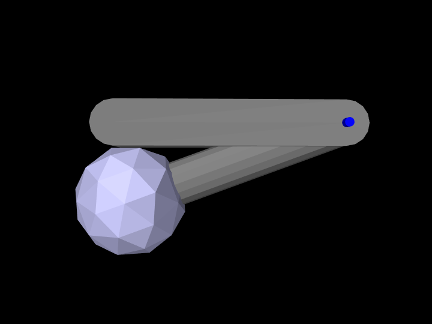
\includegraphics[]{images/JointedBallCollide}
\else
 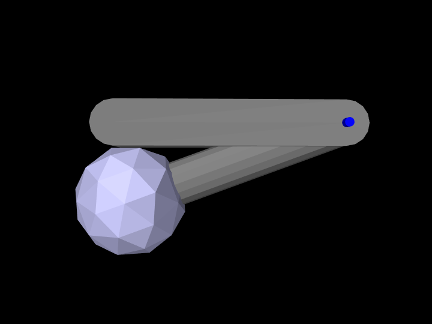
\includegraphics[width=3.75in]{images/JointedBallCollide}
\fi
\end{center}
\caption{JointedBallCollide showing the ball at the tip of 
{\tt bodyA} colliding with {\tt bodyB}.}
\label{JointedBallCollide:fig}
\end{figure}

A model illustrating how to redefine the collision mesh for a rigid
body is defined in
%
\begin{verbatim}
  artisynth.demos.tutorial.JointedBallCollide
\end{verbatim}
%
Like {\tt JointedCollide} in Section \ref{JointedCollide:sec}, this
model is simply a subclass of {\tt RigidBodyJoint} that overrides the
{\tt build()} method, adding a ball to the tip of {\tt bodyA} to
enable it to collide with {\tt bodyB}:
%
\lstset{numbers=left}
\begin{lstlisting}[]
   public void build (String[] args) {

      super.build (args); // build the RigidBodyJoint model

      // create a ball mesh
      PolygonalMesh ball = MeshFactory.createIcosahedralSphere (2.5, 1);
      // translate it to the tip of bodyA, add it to bodyA, and make it blue-gray
      ball.transform (new RigidTransform3d (5, 0, 0));
      RigidMeshComp mcomp = bodyA.addMesh (ball);
      RenderProps.setFaceColor (mcomp, new Color (.8f, .8f, 1f));

      // disable collisions for the main surface mesh of bodyA
      bodyA.getSurfaceMeshComp().setIsCollidable (false);
      // enable collisions between bodyA and bodyB
      mech.setCollisionBehavior (bodyA, bodyB, true);
   }
\end{lstlisting}
\lstset{numbers=none}

The superclass {\tt build()} method called at line 3 creates
everything contained in {\tt RigidBodyJoint}. The remaining code then
alters that model: A ball mesh is created, translated to the tip of
{\tt bodyA}, added as an additional mesh (Section
\ref{rigidBodyMultipleMeshes:sec}), and set to render as blue-gray
(lines 5-10). Next, collisions are disabled for {\tt bodyA}'s main
surface mesh by setting its {\sf isCollidable} property to {\tt false}
(line 13); this will ensure that the collision mesh associated with
{\tt bodyA} will consist solely of the ball mesh, which is necessary
because the surface mesh is permanently in contact with {\tt
bodyB}. Lastly, collisions are enabled between {\tt bodyA} and {\tt
bodyB} (line 15).

To run this example in ArtiSynth, select {\sf All demos > tutorial >
JointedBallCollide} from the {\sf Models} menu. Running the model will
cause {\tt bodyA} to fall, pivot about the hinge joint, and collide
with {\tt bodyB} (Figure \ref{JointedBallCollide:fig}).

\subsection{Compound collidables and self-collision}
\label{CompoundCollidablesAndSelf:sec}

An FEM model is an example of a {\it compound} collidable, which may
contain {\it subcollidable} descendant components which are also
collidable. Compound collidables are identified by having
their \javamethod[artisynth.core.mechmodels.Collidable]{isCompound()}
method return {\tt true}. For an FEM model, the subcollidables are the
mesh components in its {\tt meshes} list. A non-compound collidable
which is {\it not} a subcollidable of some other (compound)
collidable is called {\it solitary}. If A is a subcollidable of a
compound collidable C, then C is an {\it ancestor collidable} of A.

\begin{sideblock}
Subcollidables do not need to be immediate child components of
the compound collidable; they need only be descendants.
\end{sideblock}

One of the main purposes of compound collidables is to enable
self-collisions. While ArtiSynth does not currently support the
detection of self-collisions within a single mesh, self-collision can
be implemented within a compound collidable C by detecting collisions
amount the (separate) meshes of its subcollidables.

\begin{sideblock}
Compound collidables and their subcollidables are assumed to be
deformable; otherwise, subcollision would not be possible.
\end{sideblock}


\begin{figure}[ht]
\begin{center}
 \iflatexml
   \includegraphics[width=5in]{images/CollidableGroups}
 \else
   \includegraphics[width=5in]{images/CollidableGroups}
 \fi
\end{center}
\caption{A collection of collidable components, where A 
is compound, with subcollidables A1, A2, and A3, B is solitary, and C
is compound with subcollidables C1 and C2.  The non-compound
collidables, including the leaf nodes of the collidable trees, are
also instances of
\javaclass[artisynth.core.mechmodels]{CollidableBody},
indicated by a double outline.}
\label{CollidableGroups:fig}
\end{figure}

In general, an ArtiSynth model will contain a number of collidable
components, some of which are compound (Figure
\ref{CollidableGroups:fig}). The non-compound collidables, including
both solitary collidables and leaf nodes of a compound collidable's
tree, are also instances of the subinterface
\javaclass[artisynth.core.mechmodels]{CollidableBody}, which provide
the collision meshes, along with other information used
to compute the collision response (Section
\ref{CollidableBodies:sec}).

Actual collisions happen only between {\tt CollidableBody}s; compound
collidables are used only for determining grouping and specifying
collision behaviors. The rules for determining whether two collidable
bodies A and B will actually collide are as follows:

\begin{enumerate}

\item {\it Internal (self) collisions:}
If A and B are both subcollidables of some compound collidable C,
then A and B will collide if (a) both their {\sf collidable}
properties are set to either {\tt ALL} or {\tt INTERNAL}, and (b) an
explicit collision behavior is set between A and B, or self-collision
is enabled for C (as described below).

\item {\it External collisions:} Otherwise, if A and B are either
solitary {\it or} subcollidables of different compound collidables,
then they will collide if (a) both their {\sf collidable} properties
are set to either {\tt ALL} or {\tt EXTERNAL}, and (b) a specific or
default collision behavior is set between them or their collidable
ancestors.

\end{enumerate}

\begin{sideblock}
As mentioned above, the subcollidables of an FEM are its mesh
components (Section \ref{sec:fem:geometry}), each of which is a
collidable implemented by 
\javaclass[artisynth.core.femmodels]{FemMeshComp}.
When a mech component is added to an FEM model, using either {\tt
addMeshComp()} or one of the {\tt addMesh()} methods, its {\sf
collidable} property is automatically set to {\tt INTERNAL}, so if a
different setting is required, this must be specified {\it after} the
component has been added to the model.
\end{sideblock}

Subject to the above conditions, self-collision can be enabled for a
specific compound collidable C by calling the {\tt setCollisionBehavior()}
methods with {\tt collidable0} set to C and {\tt collidable1}
set to either C or {\tt Collidable.SELF}, as in for example:
%
\begin{lstlisting}[]
   mech.setCollisionBehavior (C, Collidable.SELF, true, mu);

   ... OR ...

   mech.setCollisionBehavior (C, C, true, mu);
\end{lstlisting}
%
It can also be enabled, by default, for all compound collidables by
calling one of the {\tt setDefaultCollisionBehavior()} methods with
{\tt collidable0} set to {\tt Collidable.DEFORMABLE} and {\tt collidable1}
set to {\tt Collidable.SELF}, e.g.:
%
\begin{lstlisting}[]
   mech.setDefaultCollisionBehavior (
      Collidable.DEFORMABLE, Collidable.SELF, true, mu);
\end{lstlisting}
%

For an example of how collision interactions can be set, refer to
Figure \ref{CollidableGroups:fig}, assume that components A, B and C
are deformable, and that the {\sf collidable} property for all
collidables is set to {\tt ALL} {\it except} for A3, where it is set
to {\tt EXTERNAL} (implying that A3 cannot self-collide with A1 and
A2). Then if {\tt mech} is the {\tt MechModel} containing the
collidables, the call
%
\begin{lstlisting}[]
   mech.setDefaultCollisionBehavior (
      Collidable.DEFORMABLE, Collidable.DEFORMABLE, true, 0.2);
\end{lstlisting}
%
will enable collisions between A1, A2, and A3 and each of B, C1, and
C2, and between B and C1 and C2, but not among A1, A2, and A3 or C1
and C2. The subsequent calls
%
\begin{lstlisting}[]
   mech.setDefaultCollisionBehavior (
      Collidable.DEFORMABLE, Collidable.SELF, true, 0);
   mech.setCollisionBehavior (B, A3, false);
\end{lstlisting}
%
will enable self-collision between A1 and A2 and C1 and C2 with zero
friction, and disable collision between B and A3.
Finally, the calls
\begin{lstlisting}[]
   mech.setCollisionBehavior (A3, C, true, 0.3);
   mech.setCollisionBehavior (A, A, false);
\end{lstlisting}
%
will enable collision between A3 and each of C1 and C2 with friction
0.3, and disable all self-collisions among A1, A2 and A3.

\subsection{Example: FEM model with self-collision}

\begin{figure}[ht]
\begin{center}
\begin{tabular}{cc}
\iflatexml
 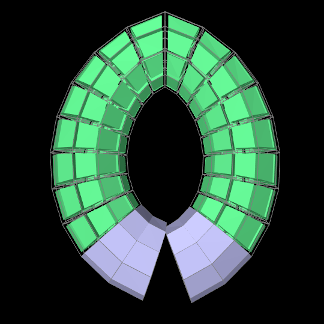
\includegraphics[]{images/FemSelfCollide}&
 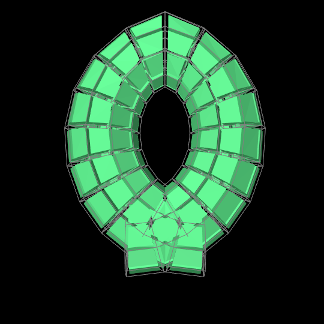
\includegraphics[]{images/FemSelfCollideOff}\\
\else
 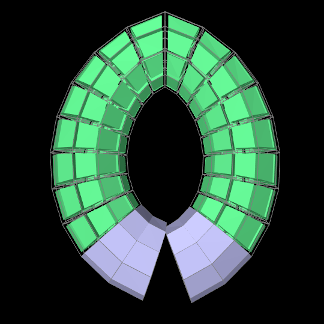
\includegraphics[width=2.25in]{images/FemSelfCollide}&
 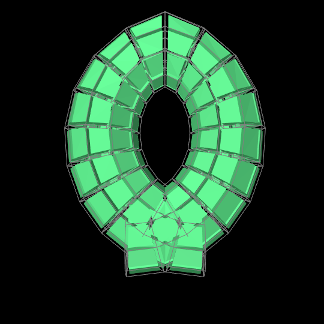
\includegraphics[width=2.25in]{images/FemSelfCollideOff}\\
\fi
\end{tabular}
\end{center}
\caption{FemSelfCollide showing collision between the left
and right contact meshes (left). Without these meshes, the FEM model
intersects with itself as show on the right.}
\label{FemSelfCollide:fig}
\end{figure}

A model illustrating self-collision for an FEM model is defined in
%
\begin{verbatim}
  artisynth.demos.tutorial.FemSelfCollide
\end{verbatim}
%
It creates a simple FEM based on a partial torus that self intersects
when it falls under gravity. Internal surface meshes are added to the
left and right ends of the model to prevent interpenetration.
The code for the {\tt build()} method is listed below:
%
\lstset{numbers=left} 
\iflatexml
%% Hack: latexml lstinputlisting doesn't handle firstline correctly
\lstset{firstnumber={-18}}
\lstinputlisting[firstline=1]{../../src/artisynth/demos/tutorial/FemSelfCollide.java}
\lstset{firstnumber={1}}
\else
\lstinputlisting[firstline=20]{../../src/artisynth/demos/tutorial/FemSelfCollide.java}
\fi
\lstset{numbers=none}

The model creates an FEM model based on an open torus, using a factory
method in \javaclass[artisynth.core.femmodels]{FemFactory}, and
rotates it so that the gap is located at the bottom (lines 7-18).  The
torus is then anchored by fixing the nodes located at the top-center
(lines 20-25). Next, mesh components are created to enforce
self-collision at the left and right gap end points (lines 27-47).
First, a \javaclass[artisynth.core.femmodels]{FemMeshComp} is created
(Section \ref{sec:fem:geometry}), and then its {\tt
createVolumetricSurface()} method is used to create a local surface
mesh wrapping the elements specified in {\tt elems}. When selecting
the elements, we use the convenient fact that for this particular FEM
model, the elements near the left and right ends have numbers in the
ranges $180 \ldots 199$ and $0 \ldots 19$, respectively.

Once the submeshes have been added to the FEM model, we create a
collision behavior and use it to enable self-collisions (lines
49-55). An explicit behavior is created so that we can enable the {\tt
VERTEX\_EDGE\_PENETRATION} contact method (Section
\ref{ContactMethods:sec}), because the meshes are coarse and the
additional edge-edge collisions will improve behavior; this method also
requires the {\tt AJL\_CONTOUR} collider type. While self-collision is
enabled by calling
%
\begin{lstlisting}[]
   mech.setCollisionBehavior (ptorus, ptorus, behav);
\end{lstlisting}
%
it could also have been enabled by calling
%
\begin{lstlisting}[]
   mech.setCollisionBehavior (ptorus, Collidable.Self, behav);

   ... OR ...

   mech.setCollisionBehavior (leftMesh, rightMesh, behav);
\end{lstlisting}
%
Note that there is no need to set the {\sf collidable} property of the
collision meshes since it is set to {\tt INTERNAL} by default when
they are added to the FEM model.

Render properties are set at lines 57-64, with the torus rendered as
light green and the collision meshes as blue-gray. The torus is drawn
using its elements widgets instead of its surface mesh, to prevent
the latter from obscuring the collision meshes.

To run this example in ArtiSynth, select {\sf All demos > tutorial >
FemSelfCollide} from the {\sf Models} menu. Running the model will
cause the FEM model to self-collide as shown in
Figure \ref{FemSelfCollide:fig}.

\subsection{Collidable bodies}
\label{CollidableBodies:sec}

As mentioned in Section \ref{CompoundCollidablesAndSelf:sec},
non-compound collidables, including both solitary collidables and leaf
nodes of a compound collidable's tree, 
are also instances of 
\javaclass[artisynth.core.mechmodels]{CollidableBody}, which
provide the actual collision meshes and other information used to
compute the collision response. This is done using various
methods, including:

\begin{itemize}

\item {\tt PolygonalMesh getCollisionMesh()}

Returns the actual surface mesh to be used for computing collisions.

\item {boolean hasDistanceGrid()}

If this method returns {\tt true}, the body also maintains a signed
distance grid for the mesh, which can be used by the collider type
{\tt SIGNED\_DISTANCE} (Section
\ref{ContactMethods:sec}).

\item {\tt DistanceGridComp getDistanceGridComp()}

If {\tt hasDistanceGrid()} returns {\tt true}, this method return the
distance grid.

\item {\tt double getMass()}

Returns the mass of this body (or a suitable estimate), for use
in automatically computing certain collision parameters.

\item {\tt int getCollidableIndex()}

Returns the index of this collidable body within the set of all {\tt
CollidableBody}s in the {\tt MechModel}. The index is determined by
the body's depth-first ordering within the model component
hierarchy. For components within the same component list, this ordering
will be determined by the order in which the components are added in
the model's {\tt build()} method.

\end{itemize}
%

\subsection{Nested MechModels}

It is possible in ArtiSynth for one {\tt MechModel} to contain other
nested {\tt MechModel}s within its component hierarchy. This raises
the question of how collisions within the nested models are
controlled. The general rule for this is the following:

\begin{sideblock}
The collision behavior for two collidables {\tt colA} and {\tt colB}
is determined by whatever behavior (either default or override) is
specified by the lowest {\tt MechModel} in the component hierarchy
that contains both {\tt colA} and {\tt colB}.
\end{sideblock}

\begin{figure}[ht]
\begin{center}
 \iflatexml
   \includegraphics[width=3.5in]{images/NestedMechCollidables}
 \else
   \includegraphics[width=3.5in]{images/NestedMechCollidables}
 \fi
\end{center}
\caption{A {\tt MechModel} containing collidables {\tt
B1} and {\tt B2}, nested within another
containing collidables {\tt A1} and {\tt A2}.}
\label{NestedMechCollidables:fig}
\end{figure}

For example, consider Figure \ref{NestedMechCollidables:fig} where we
have a {\tt MechModel} ({\tt mechB}) containing collidables {\tt B1} and
{\tt B2}, nested within another {\tt MechModel} ({\tt mechA})
containing collidables {\tt A1} and {\tt A2}. Then consider the
following code fragment:
%
\begin{lstlisting}[]
   mechB.setDefaultCollisionBehavior (true, 0.2);
   mechA.setCollisionBehavior (B1, Collidable.AllBodies, true, 0.0);
   mechA.setCollisionBehavior (B1, A1, false);
   mechA.setCollisionBehavior (B1, B2, false); // Error!
\end{lstlisting}
%
The first line enables default collisions within {\tt mechB} (with
$\mu = 0$), controlling the interaction between {\tt B1} and {\tt B2}.
However, collisions are still disabled within {\tt mechA}, meaning
{\tt A1} and {\tt A2} will not collide either with each other or with
{\tt B1} or {\tt B2}.  The second line enables collisions between {\tt
B1} and any other body within {\tt mechA} (i.e., {\tt A1} and
{\tt A2}), while the third line disables collisions between {\tt B1}
and {\tt A1}.  Finally, the fourth line results in an error, since
{\tt B1} and {\tt B2} are both contained within {\tt mechB} and so
their collision behavior cannot be controlled from {\tt mechA}.

While it is not legal to specify a specific behavior for collidables
contained in a {\tt MechModel} from a higher level {\tt MechModel},
it {\it is} legal to create collision response components for the same
pair within both models. So the following code fragment would be
allowed and would create response components in both {\tt mechA} and
{\tt mechB}:
%
\begin{lstlisting}[]
   mechB.setCollisionResponse (B1, B2);
   mechA.setCollisionResponse (B1, B2);
\end{lstlisting}
%

\section{Implementation}
\label{CollisionImplementation:sec}

This section describes the technical details of the different ways in
which collision are implemented in ArtiSynth. Knowledge of these
details can be useful for choosing collision behavior property
settings, understanding elastic foundation contact
(Section \ref{ElasticFoundationContact:sec}), and interpreting the
information provided by collision responses (Section
\ref{collisionResponse:sec}) and collision rendering (Section
\ref{ContactRendering:sec}).

The collision mechanism works by using a {\it collider} (described
further below) to locate the {\it contact regions} where the
(triangular) collision meshes of different collidables intersect
each other. Figure \ref{IntersectionRegions:fig} shows four
contact regions between two meshes representing human teeth.
Information about each contact region is then used to generate
{\it contact constraints}, according to a {\it contact method}, that
prevent further collision and resolve any existing interpenetration.

\begin{figure}[h]
\begin{center}
\iflatexml
 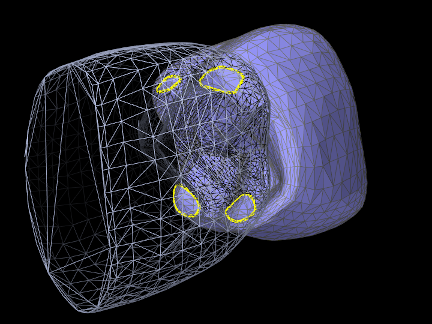
\includegraphics[]{images/molarIntersection}
\else
 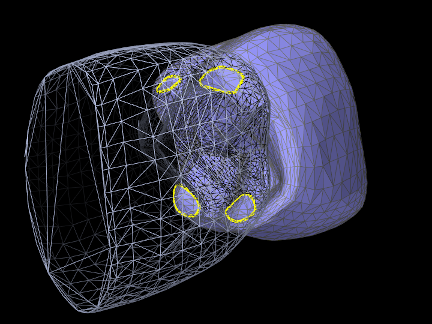
\includegraphics[width=4.5in]{images/molarIntersection}
\fi
\end{center}
\caption{Collisions between collidables are found by locating
contact regions (yellow contours) between their surface meshes.}
\label{IntersectionRegions:fig}
\end{figure}

\begin{figure}[h]
\begin{center}
\begin{tabular}{ccc}
\iflatexml
 \includegraphics[]{images/contourRegion}&
 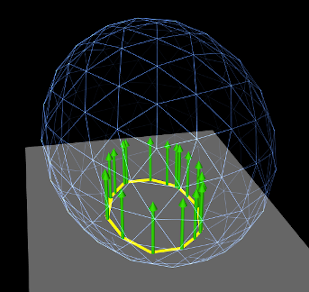
\includegraphics[]{images/contourRegionContact}\\
\else
 \includegraphics[width=3in]{images/contourRegion}&
 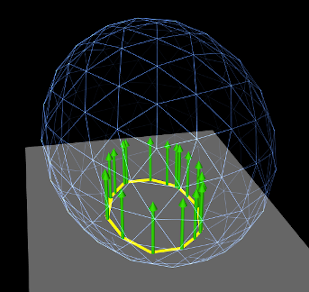
\includegraphics[width=2.5in]{images/contourRegionContact}\\
\fi
\end{tabular}
\end{center}
\caption{Contour region contact fits a plane to a contact region, and
then chooses contact points around the region's perimeter such that
their projection into the plane forms a convex hull.}
\label{ContourRegionContact:fig}
\end{figure}

\subsection{Contact methods}
\label{ContactMethods:sec}

Contact constraints are computed from mesh contact regions using
one of two primary contact methods:

\subsubsection{Contour region}
\label{ContourRegion:sec}

Contact constraints are generated for each contact region by first
fitting a plane to the region, and then selecting contact points
around its perimeter such that their 2D projection into the plane
forms a convex hull (Figure \ref{ContourRegionContact:fig}).  A
contract constraint is assigned to each contact point, with a
constraint direction parallel to the plane normal and a penetration
distance given by the maximum interpenetration of the region. Note
that the contact points do not necessarily lie {\it on} the plane, but
they all have the same normal and penetration distance.

This is the default method used between rigid bodies, since it does
not depend on mesh resolution, and rigid body contact behavior depends
only on the convex hull of the contacting regions. Since the number of
contact constraints may exceed the number of degrees of freedom (DOF)
of the contacting bodies, the constraints are supplied to the physics
solver as unilateral constraints
(Section \ref{PhysicsSimulation:sec}).  Using contact region
constraints when one of the collidables is an FEM model will result in
an error.

\subsubsection{Vertex penetration}
\label{VertexPenetration:sec}

Contacts are created for each mesh vertex that penetrates the other
mesh, with a contact normal directed toward the nearest point on the
opposing mesh (Figure \ref{VertexPenetrationContact:fig}).  Contact
constraints are generated for each contact, with the constraint
direction parallel to the normal and the penetration distance equal to
the distance to the opposing mesh.

This is the default contact method when one or both of the
collidables is an FEM model. Also by default, if only one of the
collidables is an FEM model, vertex penetrations are computed {\it
only} for the FEM collidable; penetrations of the rigid body into the
FEM are not considered. Otherwise, if both collidables are FEM models,
then vertex penetrations are computed for {\it both} bodies, resulting
in {\it two-way} contact (Figure \ref{TwoWayContact:fig}).  

Because FEM models tend to have a large number of DOFs, the default
behavior is to supply vertex penetration constraints to the physics
solver as bilateral constraints (Section \ref{PhysicsSimulation:sec}),
removing them only between simulation time steps when the contact
disappears or a separating force is detected. This results in much
faster simulation times, particularly for FEM models, because it does
not require solving a linear complementarity problem. However, this
also means that using vertex penetration between rigid bodies, or
other bodies with a low number of degrees of freedom, will typically
result in an overconstrained system that must be handled using one of
the techniques described in Section \ref{OverconstrainedContact:sec}).

\subsubsection{Setting the contact method}
\label{SettingContactMethod:sec}

Contact methods can be specified by the {\sf method} property in
either the collision manager or behavior (Section
\ref{CollisionBehavior:sec}).  The property's value is an instance of
\javaclass[artisynth.core.mechmodels]{CollisionBehavior\$Method}, for
which the standard settings are:

\begin{description}

\item[CONTOUR\_REGION]\mbox{}

Contact constraints are generated using contour regions, as described
in Section \ref{ContourRegion:sec}. Setting this for contact that
involves one or more FEM models will result in an error.

\item[VERTEX\_PENETRATION]\mbox{}

Contact constraints are generated using vertex penetration, as
described in Section \ref{VertexPenetration:sec}. Setting this for
contact between rigid bodies may result in an overconstrained system.

\item[VERTEX\_EDGE\_PENETRATION]\mbox{}

An experimental version of vertex penetration contact that
supplements vertex constraints with extra constraints formed from
edge-edge contact. Intended for collision meshes with low mesh
resolutions and sharp edges. Available only when using the {\tt
AJL\_CONTOUR} collider type (Section
\ref{ColliderTypes:sec}).

\item[DEFAULT]\mbox{}

Selects {\tt CONTOUR\_REGION} when both collidables are rigid bodies
and {\tt VERTEX\_PENETRATION} otherwise.

\item[INACTIVE]\mbox{}

No constraints are generated. This will result in no collision
response.

\end{description}

\begin{figure}[ht]
\begin{center}
\begin{tabular}{ccc}
\iflatexml
 \includegraphics[]{images/vertexPenetration}& 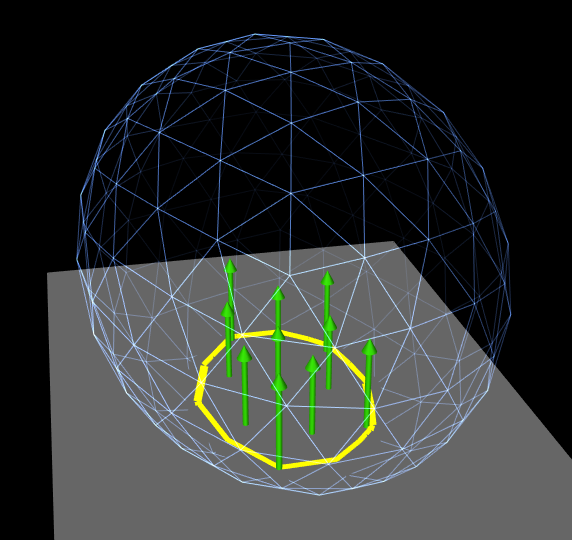
\includegraphics[]{images/vertexPenetrationContact}\\
\else
 \includegraphics[width=3in]{images/vertexPenetration}&
 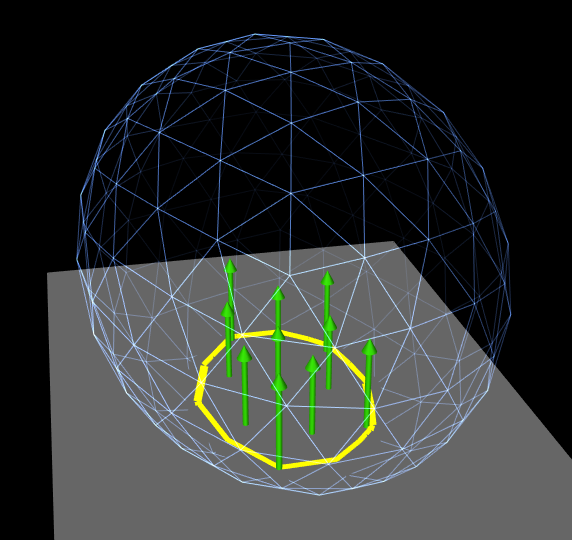
\includegraphics[width=2.5in]{images/vertexPenetrationContact}\\
\fi
\end{tabular}
\end{center}
\caption{Vertex penetration contact creates a contact point for each
penetrating vertex within a penetration region, with the contact
normal directed toward to the nearest point on the opposite mesh.}
\label{VertexPenetrationContact:fig}
\end{figure}

\begin{figure}[ht]
\begin{center}
\iflatexml
 \includegraphics[]{images/twoWayContact}
\else
 \includegraphics[width=3in]{images/twoWayContact}
\fi
\end{center}
\caption{Two-way vertex penetration contact involves creating
contact points from the penetrating vertices of {\it both}
meshes.}
\label{TwoWayContact:fig}
\end{figure}

When vertex penetration contact is employed, the collidables for which
penetrations are generated can also be controlled using the {\sf
vertexPenetrations} property, whose value is an instance of
\javaclass[artisynth.core.mechmodels]{CollisionBehavior\$VertexPenetrations}:

\begin{description}

\item[BOTH\_COLLIDABLES]\mbox{}

Vertex penetrations are computed for both collidables.

\item[FIRST\_COLLIDABLE]\mbox{}

Vertex penetrations are computed for the first collidable.

\item[SECOND\_COLLIDABLE]\mbox{}

Vertex penetrations are computed for the second collidable.

\item[AUTO]\mbox{}

Vertex penetrations are determined automatically as follows: for both
collidables if neither is a rigid body, for the non-rigid collidable
if one collidable is a rigid body, and for the first collidable
otherwise.

\end{description}

\subsection{Collider types}
\label{ColliderTypes:sec}

The contact regions used by the contact method are generated by
a collider, which is specified by the {\sf colliderType} property in
either the collision manager (as the default), or in the collision
behavior for a specific pair of collidables. The property's value is an
instance of
\javaclass[artisynth.core.mechmodels]{CollisionManager\$ColliderType},
which describes the three collider types presently supported:

\begin{description}

\item[TRI\_INTERSECTION]\mbox{}

The original ArtiSynth collider which uses a bounding-box hierarchy to
locate all triangle intersections between the two surface
meshes. Contact regions are then estimated by grouping the
intersection points together, and penetrating vertices are computed
separately using point-mesh distance queries based on the bounding-box
hierarchy. This latter step requires iterating over all mesh vertices,
which may be slow for large meshes. {\tt TRI\_INTERSECTION} can often
handle intersections near the edges of an open mesh, but does not
support the {\tt VERTEX\_EDGE\_PENETRATION} contact method.

\item[AJL\_CONTOUR]\mbox{}

A bounding-box hierarchy is used to locate all triangle intersections
between the two surface meshes, and the intersection points are then
connected, using robust geometric predicates, to find the (piecewise
linear) intersection contours.  The contours are then used to identity
the contact regions on each surface mesh, which are in turn used to
determine the interpenetrating vertices and contact area. Intersection
contours and the contact constraints generated from them are shown in
Figure~\ref{Collision:fig}.  {\tt AJL\_CONTOUR} supports the {\tt
VERTEX\_EDGE\_PENETRATION} contact method, but usually {\it cannot}
handle intersections near the edges of an open mesh.

\item[SIGNED\_DISTANCE]\mbox{}

Uses a grid-based signed distance field on one mesh to quickly
determine the penetrating vertices of the opposite mesh, along with
the penetration distance and normals.  This is only available for
collidable pairs where at least one of the bodies maintains a signed
distance grid which can be obtained using
\javamethod[artisynth.core.mechmodels.CollidableBody]{getDistanceGridComp()}.
Advantages include speed (sometimes an order of magnitude faster than
the other colliders) and the fact that the opposite mesh does {\it
not} have to be triangular or manifold.  However, signed distance
fields can (at present) only be computed for fixed meshes, and so at
least one colliding body must be rigid.  The signed distance field
also does not yet yield contact region information, and so the
contact method is restricted to
\javaclassAlt{%
artisynth.core.mechmodels.CollisionBehavior\$Method\#VERTEX\_PENETRATION}%
{VERTEX\_PENETRATION}.
Contacts generated from a signed distance field are illustrated in
Figure Figure~\ref{SDCollision:fig}.

\begin{sideblock}
Because the {\tt SIGNED\_DISTANCE} collider type currently supports
only the {\tt VERTEX\_PENETRATION} method, its use between rigid
bodies, or low DOF deformable bodies, will generally result in an
overconstrained system unless measures are taken as described in
Section \ref{OverconstrainedContact:sec}.
\end{sideblock}

\end{description}

\begin{figure}[ht]
\begin{center}
        \begin{tabular}{ccc}
        \includegraphics[width=0.31\textwidth]{images/femCollide1} &
        \includegraphics[width=0.31\textwidth]{images/femCollide2} &
        \includegraphics[width=0.31\textwidth]{images/femCollide3}\\
%       \end{tabular}
%       \begin{tabular}{p{1.2cm}p{3.5cm}p{3.5cm}p{3.5cm}} 
         \large  $\mathrm{t}=0$s & \large $\mathrm{t}=0.25$s & \large $\mathrm{t}=0.5$s         
        \end{tabular}
\end{center}
\caption{Time sequence of contact handling between two deformable models 
falling under gravity, 
showing the intersection contours
(yellow) and the contact normals (green lines).}
\label{Collision:fig}
\end{figure}

\begin{figure}[ht]
\begin{center}
     \includegraphics[width=0.5\textwidth]{images/signedDistanceCollide}
\end{center}
\caption{Contacts generated by a signed distance field. A deformable
ellipsoid (red, top) is colliding with a solid prism (cyan, bottom).
A signed distance field for the prism (the grid points and normals of
which are shown partially by the dark cyan arrows) is used to locate
penetrating vertices of the ellipsoid and hence generate contact
constraints (yellow lines).}
\label{SDCollision:fig}
\end{figure}

\subsubsection{Collision meshes and signed distance grids}
\label{collisionMeshes:sec}

As described in Section \ref{CollidableBodies:sec}, collidable bodies
declare the method
\javamethod[artisynth.core.mechmodels.CollidableBody]{getCollisionMesh()},
which returns a mesh defining the collision surface.  This is either
used directly, or, for the {\tt SIGNED\_DISTANCE} collider, used
to compute a signed distance grid which in turn in used to handle
collisions.

For \javaclass[\mech]{RigidBody} objects, the mesh returned by {\tt
getCollisionMesh()} is typically the same as the surface mesh.
However, it is possible to change this, by adding additional meshes to
the body and modifying the meshes' {\sf isCollidable} property (see
Section
\ref{CollisionMeshesAndCompounds:sec}). The collision mesh is then formed
as the sum of all polygonal meshes in the body's {\tt meshes} list
whose {\sf isCollidable} property is {\tt true}.

Collidable bodies also declare the methods
\javamethod[artisynth.core.mechmodels.CollidableBody]{hasDistanceGrid()}
and
\javamethod[artisynth.core.mechmodels.CollidableBody]{getDistanceGridComp()}.
If the former returns {\tt true}, then the body has a distance grid
and the latter returns a \javaclass[\mech]{DistanceGridComp}
containing it.  A distance grid is a regular 3D grid, with uniformly
arranged vertices and cells, that is used to represent a scalar
distance field, with distance values stored implicitly at each vertex
and interpolated within cells. Distance grids are used by the {\tt
SIGNED\_DISTANCE} collider, and by default are generated
on-demand, using an automatically chosen resolution and the mesh
returned by
\javamethod[artisynth.core.mechmodels.CollidableBody]{getCollisionMesh()}
as the surface against which distances are computed.

When used for collision handling, values within a distance grid are
interpolated trilinearly within each cell. This means that the
effective collision surface is actually the trilinearly interpolated
isosurface corresponding to a distance of 0. This surface will differ
somewhat from the original surface returned by {\tt
getCollisionMesh()}, in a manner that depends on the grid resolution.
Consequently, when using the {\tt SIGNED\_DISTANCE} collider, it
is important to be able to visualize the trilinear isosurface, and
possibly modify it by adjusting the grid resolution. The {\tt
DistanceGridComp} returned by {\tt getDistanceGridComp()} exports
properties to facilitate both of these requirements, as described in
detail in Section \ref{DistanceGrids:sec}.

\section{Contact rendering}
\label{ContactRendering:sec}

As mentioned in Section \ref{CollisionBehavior:sec}, additional
collision behavior properties exist to enable and control the
rendering of contact artifacts. These include intersection contours,
contact points and normals, contact forces and pressures, and
penetration depths. The properties that control these are supplemented
by generic render properties (Section \ref{RenderProperties:sec}) to
specify colors, line widths, etc. 

By default, contact rendering is disabled. To enable it, one must set
the collision manager to be {\it visible}, which can be done using a code
fragment like the following:
%
\begin{verbatim}
  RenderProps.setVisible (mechModel.getCollisionManager(), true);
\end{verbatim}
%

\javaclass[artisynth.core.mechmodels]{CollisionManager} and
\javaclass[artisynth.core.mechmodels]{CollisionBehavior}
both export contact rendering properties. Setting these in the former
controls rendering globally for all collisions, while setting them in
the latter controls rendering for the collidable pair associated with
the behavior.  Some artifacts, like contact normals, forces, and color
maps, must be drawn with respect to either the first or second
collidable. By default, the first collidable is chosen, but the second
collidable can be requested using the {\sf renderingCollidable}
property described below. Normals are drawn {\it toward}, and forces
drawn such that they are acting {\it on}, the indicated
collidable. For collision behaviors specified using the {\tt
setCollisionBehavior()} methods, the first and second collidables
correspond to the {\tt collidable0} and {\tt collidable1} arguments.
Otherwise, for default collision behaviors, the first collidable will
be the one whose collidable bodies have the lowest collidable index
(Section \ref{CollidableBodies:sec}).

Properties exported by both {\tt CollisionManager} and {\tt
CollisionBehavior} include:

\begin{description}

\item[renderingCollidable]\mbox{}

Integer value of either 0 or 1 specifying the collidable for which
forces, normals and color maps should be drawn. 0 or 1 selects either
the first or second collidable. The default value is 0.

\item[drawIntersectionContours]\mbox{}

Boolean value requesting drawing of the intersection contours between
collidable meshes, using the generic render properties {\sf edgeWidth}
and {\sf edgeColor}. The default value is {\tt false}.

\item[drawIntersectionPoints]\mbox{}

Boolean value requesting drawing of the interpenetrating vertices on
each collidable mesh, using the generic render properties {\sf
pointStyle}, {\sf pointSize}, {\sf pointRadius}, and {\sf pointColor}.
The default value is {\tt false}.

\item[drawContactNormals]\mbox{}

Boolean value requesting drawing of the normals associated with each
contact constraint, using the generic render properties {\sf
lineStyle}, {\sf lineRadius}, {\sf lineWidth}, and {\sf lineColor}.
The default value is {\tt false}. The length of the normals is
controlled by the {\sf contactNormalLen} property of the collision
manager, which will be set to an appropriate default value if not set
explicitly.

\item[drawContactForces]\mbox{}

Boolean value requesting drawing of the forces associated with each
contact constraint, using the generic render properties {\sf
lineStyle}, {\sf lineRadius}, {\sf edgeWidth}, and {\sf edgeColor} (or
{\sf lineColor} if {\sf edgeColor} is {\tt null}).  The default value
is {\tt false}. The forces are drawn as line segments starting at each
contact point and running parallel to the contact normal, with a
length given by the current contact impulse value multiplied by the
{\sf contactForceLenScale} property of the collision manager (which
has a default value of 1).  The reason for using {\sf edgeWidth} and
{\sf edgeColor} instead of {\sf lineWidth} and {\sf lineColor} is to
allow the application to set the render properties such that both
normals and forces can be visible if both are being rendered at the
same time.

\item[drawFrictionForces]\mbox{}

Boolean value requesting the drawing of the forces associated with
each contact's friction force, in the same manner and style as for
{\sf drawContactForces}. The default value is {\tt false}. Note that
unlike contact forces, friction forces are {\it perpendicular} to the
contact normal.

\item[drawColorMap]\mbox{}

An enum of type
\javaclass[artisynth.core.mechmodels]{CollisionBehavior\$ColorMapType}
requesting that a color map be drawn over the contact regions showing
a scalar value such as penetration depth or contact force pressure.
The collidable (0 or 1) onto which the color map is drawn is
controlled by the {\sf renderingCollidable} property (described
below). The range of values used for generating the map is controlled
by the {\sf colorMapRange} property of either the collision manager or
the behavior, as described below.  The values are mapped onto colors
using the {\sf colorMap} property of the collision manager.

Values of
\javaclass[artisynth.core.mechmodels]{CollisionBehavior\$ColorMapType}
include:

\begin{description}

\item[NONE]\mbox{}

The color map is disabled. This is the default value.

\item[PENETRATION\_DEPTH]\mbox{}

The color map shows penetration depth of one collidable mesh with
respect to the other. If one or both collidable meshes are open, then
the {\sf colliderType} should be set to {\tt AJL\_CONTOUR} (Section
\ref{CollisionBehavior:sec}).

\item[CONTACT\_PRESSURE]\mbox{}

The color map shows the contact pressures over the contact region.
Contact pressures are determined by examining the forces at the
contact constraints and then distributing these over the surrounding
faces. This information is most useful and accurate when using
vertex penetration contact (Section \ref{VertexPenetration:sec}).

\end{description}

The color map itself is drawn as a patch formed from the collidable's
collision mesh, using faces and vertices associated with the collision
region. The vertices of the patch are set to colors corresponding to
the associated value (e.g., penetration depth or pressure) at that
vertex, and the surrounding faces are colored appropriately.  The
resolution of the color map is thus determined by the resolution of
the collision mesh, and so the application must ensure this is high
enough to ensure proper results. If the mesh has only a few triangles
(e.g., a rectangle with two triangles per face), the color
interpolation may be spread over an unreasonably large area.  Examples
of color map usage are given in Sections \ref{renderingDepth:sec} and
\ref{renderingContactPressure:sec}.

\item[colorMapRange]\mbox{}

Composite property of the type
\javaclass[artisynth.core.util]{ScalarRange} that controls the range
of values used for color map rendering. Subproperties include {\sf
interval}, which gives the value range itself, and {\sf updating},
which specifies how this interval should be updated: {\tt FIXED} (no
updating), {\tt AUTO\_EXPAND} (interval is expanded as values increase
or decrease), and {\tt AUTO\_FIT} (interval is reset to fit the values
at every render step).

When the {\sf colorMapRange} value for a {\tt CollisionBehavior} is
set to {\tt null} (which is the default), the {\sf colorMapRange} of
the {\tt CollisionManager} is used instead. This has the advantage of
ensuring that the same color map range will be used across all
collision interactions.

\item[colorMapInterpolation]\mbox{}

An enum of type
\javaclass[maspack.render]{Renderer\$ColorInterpolation} that explicitly
specifies how colors in any rendered color map should be interpolated.
{\tt RGB} and {\tt HSV} (the default) specify interpolation in RGB and
HSV space, respectively. HSV interpolation is the default as it is
generally better suited to rendering maps that are purely color-based.

\end{description}

In addition, the following properties are exported by the collision
manager:

\begin{description}

\item[contactNormalLen]\mbox{}

Double value specifying the length with which contact normals should
be drawn when {\sf drawContactNormals} is {\tt true}. If unspecified,
a default value is calculated by the system.

\item[contactForceLenScale]\mbox{}

Double value specifying the scaling factor for contact or friction
force vectors when they are drawn in response to {\sf
drawContactForces} {\sf drawFrictionForces} being {\tt true}.  The
default value is 0.

\item[colorMap]\mbox{}

Composite property of type 
\javaclass[maspack.render.color]{ColorMapBase} 
specifying the actual color map used for color map rendering.
The default value is 
\javaclass[maspack.render.color]{HueColorMap}.

\end{description}


Generic render properties within the collision manager can be
set in the same way as the visibility, using the {\tt RenderProps}
methods presented in Section \ref{SettingRenderProperties:sec}:
\begin{lstlisting}[]
  Renderable cm = mechModel.getCollisionManager();
  RenderProps.setEdgeWidth (cm, 2);
  RenderProps.setEdgeColor (cm, Color.Red);
\end{lstlisting}

As mentioned above, generic render properties can also be set
individually for specific behaviors. This can be done using code
fragments like this:
\begin{lstlisting}[]
  CollisionBehavior behav = mechModel.getCollisionBehavior (bodA, bodB);
  RenderProps.setLineWidth (behav, 2);
  RenderProps.setLineColor (behav, Color.Blue);
\end{lstlisting}
To access these properties on a read-only basis, one can do
\begin{lstlisting}[]
  RenderProps props = mechModel.getCollisionManager().getRenderProps();

  ... OR ...

  RenderProps props = behav.getRenderProps();
\end{lstlisting}

\begin{sideblock}
Because of the manner in which ArtiSynth handles contacts, rendered
contact information may sometimes appear to lag the simulation by one
time step. That is because contacts are computed at the {\it end} of
each time step $i$, and then used to compute the contact forces during
the next step $i+1$. The contact information displayed at the end of
step $i$ is thus based on contacts detected at the end of step $i-1$,
along with contact forces that are computed during step $i$ and used to
calculate the updated positions and velocities at the end of that step.
\end{sideblock}

\subsection{Example: rendering normals and contours}
\label{RenderingContactNormals:sec}

A simple model illustrating contact rendering is defined in
%
\begin{verbatim}
  artisynth.demos.tutorial.BallPlateCollide
\end{verbatim}
%
This shows a ball colliding with a plate, while rendering the
resulting contact normals in red and the intersection contours in
blue. This demo also allows the user to experiment with compliant
contact (Section \ref{CompliantContact:sec}) by setting
{\sf compliance} and {\sf damping} properties in a control panel.

\begin{figure}[ht]
\begin{center}
\iflatexml
 \includegraphics[]{images/BallPlateCollide}
\else
 \includegraphics[width=3.25in]{images/BallPlateCollide}
\fi
\end{center}
\caption{BallPlateCollide showing contact normals (red) and collision contour
(blue) of the ball colliding with the plate.}
\label{BallPlateCollide:fig}
\end{figure}

The complete source code is shown below:
%
\lstset{numbers=left}
\lstinputlisting{../../src/artisynth/demos/tutorial/BallPlateCollide.java}
\lstset{numbers=none}

The {\tt build()} method starts by creating and adding a {\tt
MechModel} in the usual way (lines 19-20). The ball and plate are both
created as rigid bodies (lines 22-28), with the ball pose set so that
its origin is above the plate at (0, 0, 2) and its orientation is
perturbed so that it will not land on the plate symmetrically (line
24). Collisions between the ball and plate are enabled at line 31, with
a friction coefficient of 0.2. To allow better visualization of the
contacts, the ball is made transparent by disabling the drawing of
faces, and instead enabling the drawing of edges in white with no
shading (lines 33-37).

Rendering of contacts and normals is established by setting the render
properties of the collision manager (lines 39-47). First, the
collision manager is set visible (which it is not by default).  Then
lines (used to render the contact normals) and edges (used to render
to intersection contour) are set to red and blue, each with a pixel
width of 3.  Drawing of the normals and contour is enabled at lines
46-47.

Lastly, for interactively controlling contact compliance
(Section \ref{CompliantContact:sec}), a control panel is built to
allow users to adjust the collision manager's {\sf compliance} and
{\sf damping} properties (lines 49-53).

To run this example in ArtiSynth, select {\sf All demos > tutorial >
BallPlateCollide} from the {\sf Models} menu. When run, the ball
will collide with the plate and the contact normals and collision 
contours will be drawn as shown in Figure \ref{BallPlateCollide:fig}.

To enable compliant contact, set the {\sf compliance} to a
non-zero value. A value of 0.001 (which corresponds to a contact
stiffness of 1000) causes the ball to bounce considerably when it
lands. To counteract this bouncing, the {\sf damping} should be set to
a non-zero value. Since the ball has a mass of ~0.21, formula
(\ref{contactDamping:eqn}) suggests that critical damping (for which
$\zeta=1$) can be achieved with $D \approx 30$. This does in fact stop
the bouncing. Increasing the compliance to 0.01 results in the ball
penetrating the plate by a noticeable amount.

\subsection{Example: rendering a color map}
\label{renderingDepth:sec}

As described above, it is possible to use the {\sf drawColorMap}
property of the collision behavior to render a color map over the
contact area showing a scalar value such as penetration depth or
contact pressure. A simple example of this is defined in
%
\begin{verbatim}
  artisynth.demos.tutorial.PenetrationRender
\end{verbatim}
%
which sets {\sf drawColorMap} to {\tt PENETRATION\_DEPTH} in order to
display the penetration depth of one hemispherical mesh with respect
to another. 

\begin{sideblock}
As mentioned above, proper results require that the collision mesh for
the collidable on which the map is being drawn has a sufficiently high
resolution.
\end{sideblock}

\begin{figure}[ht]
\begin{center}
\iflatexml
 \includegraphics[]{images/PenetrationRender}
\else
 \includegraphics[width=3.75in]{images/PenetrationRender}
\fi
\end{center}
\caption{PenetrationRender showing the penetration depth of the bottom
mesh with respect to the top, with red indicating greater depth.
A translation dragger fixture at the top is being used to 
move the top mesh around, while the penetration range and
associated colors are displayed on the color bar at the right.}
\label{PenetrationRender:fig}
\end{figure}

The complete source code is shown below:
%
\lstset{numbers=left}
\lstinputlisting{../../src/artisynth/demos/tutorial/PenetrationRender.java}
\lstset{numbers=none} 

To improve visibility, the example uses two rigid bodies, each created
from an open hemispherical mesh using the method {\tt
createHemiBody()} (lines 32-47). Because this example is strictly
graphical, the bodies are set to be non-dynamic so that they can be
moved around using the viewer's graphical dragger fixtures (see the
section ``Transformer Tools'' in the
\artisynthManual{uiguide}{ArtiSynth User Interface Guide}). 
Rendering properties for each body are set at lines
67-68 and 73-76, with the top body being rendered as a wireframe to
improve visibility.

Lines 80-84 create and set a collision behavior between the two bodies
with the {\sf drawColorMap} property set to
{\tt PENETRATION\_DEPTH}. Because for this example we
want to show only the penetration and don't want a collision response,
we set the contact method to be \javaclassAlt{%
artisynth.core.mechmodels.CollisionBehavior\$Method\#INACTIVE}%
{Method.INACTIVE}.
At line 88, the collider type used by the collision manager is set to
\javaclassAlt{%
artisynth.core.mechmodels.CollisionManager\$ColliderType\#AJL\_CONTOUR}%
{ColliderType.AJL\_CONTOUR}, since this provides more reliable
penetration calculations for open meshes.  Other rendering properties
are set for the collision manager at lines 90-107, including a custom
color map that varies between {\tt CREAM} (the color of the mesh) for
no penetration and dark red for maximum penetration. The updating of
the color map range in the collision manager is set to {\tt AUTO\_FIT}
so that it will be recomputed at every time step. (Since the collision
manager's color map range is set to ``auto fit'' by default, this is
shown for illustrative purposes only. It is also possible to override
the collision manager's color map range by setting the {\sf
colorMapRange} property in specific collision behaviors.)

At line 111, a color bar is created and added to the scene, using the
method {\tt createColorBar()} (lines 50-59), to explicitly show the
depth that corresponds to the different colors. The color bar is given
the same color map that is used to render the depth. Since the depth
range is updated every time step, it is also necessary to update the
corresponding labels in the color bar. This is done by overriding the
root model's {\tt prerender()} method (lines 115-132), where we obtain
the color map range for the collision manager and use it to update the
color bar labels. (Note that {\tt super.prerender(list)} is called {\it
first}, since the color map ranges are updated there.)
References to the color bar, {\tt MechModel}, and
bodies are obtained using the
\javaclass[artisynth.core.modelbase]{CompositeComponent} methods
\javamethod*[artisynth.core.modelbase.CompositeComponent]{get()} and
\javamethod*[artisynth.core.modelbase.CompositeComponent]{findComponent()}.
This is more robust that storing these references in  member
variables, since the latter would be lost if the model is saved to and
reloaded from a file.

To run this example in ArtiSynth, select {\sf All demos > tutorial >
PenetrationRender} from the {\sf Models} menu. When run, the meshes
will collide and render the penetration depth of the bottom mesh, 
as shown in Figure \ref{PenetrationRender:fig}.

\begin{sideblock}
When defining the color map for rendering (lines 99-108 in the
example), it is recommended that the color corresponding to zero be
set to the face color of the collidable mesh.  This will allow
the color map to blend properly to the regular mesh color.
\end{sideblock}

\subsection{Example: rendering contact pressures}
\label{renderingContactPressure:sec}

Color map rendering can also be used to render contact pressures,
which can be particularly useful for FEM models. A simple example is
defined in
%
\begin{verbatim}
  artisynth.demos.tutorial.ContactPressureRender
\end{verbatim}
%
which sets the {\sf drawColorMap} property of the collision behavior to {\tt
CONTACT\_PRESSURE} in order to display a color map of the contact
pressure. The example is similar to that
of Section \ref{renderingDepth:sec}, which shows how to render
penetration depth.

\begin{sideblock}
The caveats about color map rendering described in Section
\ref{ContactRendering:sec} apply. 
Pressure rendering is most useful and accurate when using vertex penetration
contact. The resolution of the color map is limited by
the resolution of the collision mesh for the collidable on which the
map is drawn, and so the application should ensure that this is
sufficiently fine. Also, to allow the map to blend properly with the
rest of the collidable, the color corresponding to zero pressure
should match the default face color for the collidable.
\end{sideblock}

\begin{figure}[ht]
\begin{center}
\iflatexml
 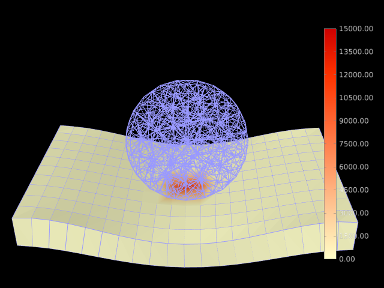
\includegraphics[]{images/ContactPressureRender}
\else
 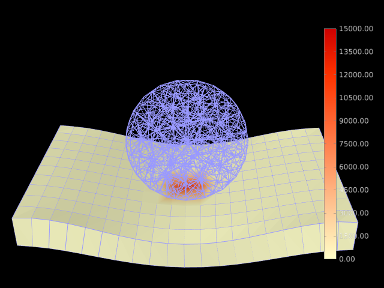
\includegraphics[width=3.75in]{images/ContactPressureRender}
\fi
\end{center}
\caption{ContactPressureRender showing the contact pressure as a
spherical FEM model falls onto an FEM sheet.  The color map is drawn
on the sheet model, with redder values indicating greater pressure.}
\label{ContactPressureRender:fig}
\end{figure}

The complete source code is shown below:
%
\lstset{numbers=left}
\lstinputlisting{../../src/artisynth/demos/tutorial/ContactPressureRender.java}
\lstset{numbers=none} 

To begin, the demo creates two FEM models: a spherical ball (lines
52-56) and a rectangular sheet (lines 59-66), and then fixes the end
nodes of the sheet (lines 69-74). Surface rendering is enabled for
the sheet (line 65), but not for the ball, in order to improve the
visibility of the color map.

Lines 77-81 create and set a collision behavior between the two
models, with the {\sf drawColorMap} property set to {\tt
CONTACT\_PRESSURE}. Because for this example we want the color map to
be drawn on the {\it second} collidable (the sheet), we set the {\sf
setColorMapCollidable} property to 1 (line 79); otherwise, the default
value of 0 would cause the color map to be drawn on the first
collidable (the ball). (Alternatively, we could have simply defined
the collision behavior as being between the surface and the ball
instead of the ball and the sheet.) The color map range is explicitly
set to lie between $[0, 15000]$ (line 80); this is in contrast to the
example in Section \ref{renderingDepth:sec}, where the range is
auto-updated on each step. The color range is also set explicitly in
the behavior, but if multiple objects were colliding it would likely
be preferable to set it in the collision manager (with the behavior's
value left as {\tt null}) to ensure a uniform render range across all
collisions.  Other rendering properties are set for the collision
manager at lines 83-97, including a custom color map that varies
between {\tt CREAM} (the color of the mesh) for no pressure and dark
red for maximum pressure.

At line 100, a color bar is created and added to the scene, using the
method {\tt createColorBar()} (lines 36-45), to explicitly show the
pressure that corresponds to the different colors. The color bar is
given the same color map and value range used to render the
pressure. Finally, default face and line colors for all components in
the model are set at lines 105-106.

To run this example in ArtiSynth, select {\sf All demos > tutorial >
ContactPressureRender} from the {\sf Models} menu. When run, the FEM
models will collide and render the contact pressure on the sheet, as
shown in Figure \ref{ContactPressureRender:fig}.

\section{Overconstrained contact}
\label{OverconstrainedContact:sec}

When contact occurs between collidable bodies, the system creates a
set of contact constraints to handle the collision and passes these to
the physics solver (Section \ref{PhysicsSimulation:sec}).  When one or
both of the contacting collidables are FEM models, the number of
constraints is usually less than the DOF count of the collidables.
However, if the both collidables are rigid bodies, then the number of
constraints often {\it exceeds} the DOF count, a situation which is
referred to as {\it redundant contact}. Redundant contact can also
occur in other collision situations, such those involving embedded
meshes (Section \ref{FEMmeshEmbedding:sec}) when the mesh has a finer
resolution than the embedding FEM, or skinned meshes
(Chapter \ref{skinning:sec}) when the number of contacts exceeds the
DOF count of the underlying master bodies.

Redundant contact is not usually a problem in collisions between rigid
bodies, because by default ArtiSynth handles these using {\tt
CONTOUR\_REGION} contact (Section \ref{ContactMethods:sec}), for
which contacts are supplied to the physics solver as {\it unilateral}
constraints which are solved using complementarity techniques
that can handle redundant constraints. However, as mentioned in
Section \ref{VertexPenetration:sec}, the default implementation for
vertex penetration contact is to present the contacts to the
physics solver as {\it bilateral} constraints (Section
\ref{PhysicsSimulation:sec}), which are removed between simulation
steps. This results in much faster simulation times, and usually works
well in the case of FEM models, where the DOF count almost always
exceeds the number of constraints. However, when vertex penetration
contact is employed between rigid bodies, and sometimes in other
situations as described above, redundant contact can arise, and then
the use of bilateral constraints results in {\it overconstrained
contact} for which the solver has difficulty finding a proper
solution.

A common indicator of overconstrained contact is for an error message
to appear in ArtiSynth's console output, which typically looks like
this:
%
\begin{verbatim}
  Pardiso: num perturbed pivots=12
\end{verbatim}
%
The simulation may also go unstable.

At present there are three general ways to manage overconstrained
contact: 

\begin{enumerate}

\item Requiring the system to use {\it unilateral} constraints for
vertex penetration contact. This can be done by setting the
property {\sf bilateralVertexContact} (Section
\ref{CollisionBehavior:sec}) to {\tt false} in either the collision
manager or behavior, but the resulting hit to computational
performance may be large.

\item Constraint reduction, described in Section
\ref{ConstraintReduction:sec}.

\item Regularizing the contact, using one of the methods
of Section \ref{ContactRegularization:sec}.

\end{enumerate}

\begin{sideblock}
When using the new implicit friction integration feature (Section
\ref{FrictionAndStability:sec}), if redundant contacts arise, it is
necessary to regularize both the contact constraints, as per Section
\ref{ContactRegularization:sec}, as well as the friction constraints,
by setting the {\sf stictionCreep} property of either the collision
manager or behavior to a non-zero value, as described in Section
\ref{CollisionBehavior:sec}.
\end{sideblock}

\subsection{Constraint reduction}
\label{ConstraintReduction:sec}

Constraint reduction involves having the collision manager explicitly
try to reduce the number of collision constraints to match the
available DOFs, and is enabled by setting the {\sf reduceConstraints}
property for either the collision manager
{\it or} the \javaclass[artisynth.core.mechmodels]{CollisionBehavior}
for a particular collision pair to {\tt true}. The default value of
{\sf reduceConstraints} is {\tt false}. As with all properties, it can
be set interactively in the GUI, or in code using the property's
accessor methods,
%
\begin{lstlisting}[]
  boolean getReduceContraints()
  void setReduceContraints (boolean enable)
\end{lstlisting}
%
as illustrated by the following code fragments:
%
\begin{lstlisting}[]
  MechModel mech;
  ...

  // enable constraint reduction for all collisions:
  mech.getCollisionManager().setReduceContraints (true);

  // enable constraint reduction for collisions between bodyA and bodyB:
  CollisionBehavior behav = 
     mech.setCollisionBehavior (bodyA, bodyB, true);
  behav.setReduceContraints (true);
\end{lstlisting}
%

\section{Contact regularization}
\label{ContactRegularization:sec}

Contact regularization is a technique in which contact
constraints are made ``soft'' by adding compliance and damping.  This
means that they no longer remove DOFs from the system, and so
overconstraining cannot occur, but contact penetration is no longer
strictly enforced and there may be an increase in the computation time
required for the simulation. 

\subsection{Compliant contact}
\label{CompliantContact:sec}

Compliant contact is a simple form of regularization that is analogous
to that used for joints and connectors, discussed in Section
\ref{JointCompliance:sec}.  Compliance and damping parameters $C$ and
$D$ can be specified between any two collidables, with $C$ being the
{\it inverse} of a corresponding contact stiffness $K = 1/C$, such the
contact forces $f_c$ acting along each contact normal are given by
%
\begin{equation}
f_c = - K d - D \dot d,
\label{contactForce:eqn}
\end{equation}
%
where $d$ is the contact penetration distance and is {\it negative}
when penetration occurs. Contact forces act to push the contacting
bodies apart, so if body A is penetrating body B and the contact
normal $\n$ is directed {\it toward} A, the forces acting on A and B
at the contact point will be $f_c \n$ and $-f_c \n$, respectively.
Since $C$ is the inverse of the contact stiffness $K$, a value of $C =
0$ (the default) implies ``infinitely'' stiff contact
constraints. Compliance is enabled whenever the compliance is set
to a value greater than 0, with stiffness decreasing as compliance
increases.

Compliance can be enabled by setting the {\sf compliance} and {\sf
damping} properties of either the collision manager {\it or} the
\javaclass[artisynth.core.mechmodels]{CollisionBehavior} for a
specific collision pair; these properties correspond to $C$ and $D$ in
(\ref{contactForce:eqn}). While it is not required to set the damping
property, it is usually desirable to set it to a value that
approximates critical damping in order to prevent ``bouncing'' contact
behavior. Compliance and damping can be set in the GUI by editing the
properties of either the collision manager or a specific collision
behavior, or set in code using the accessor methods
%
\begin{lstlisting}[]
  double getCompliance()
  void setCompliance (double c)

  double getDamping()
  void setDamping (double d)
\end{lstlisting}
%
as is illustrated by the following code fragments:
%
\begin{lstlisting}[]
  MechModel mech;
  double compliance;
  double damping;

  ... determine compliance and damping values ...

  // set damping and compliance for all collisions:
  mech.getCollisionManager().setCompliance (compliance);
  mech.getCollisionManager().setDamping (damping);

  // enable compliance and damping between bodyA and bodyB:
  CollisionBehavior behav = 
     mech.setCollisionBehavior (bodyA, bodyB, true);
  behav.setCompliance (compliance);
  behav.setDamping (damping);
\end{lstlisting}
%

An important question is what values to choose for compliance and
damping. At present, there is no automatic way to determine these, and
so some experimental parameter tuning is often necessary. With regard
to the contact stiffness $K$, appropriate values will depend on the
desired maximum penetration depth and other loadings acting on the
body. The mass of the collidable bodies may also be relevant if one
wants to control how fast the contact stabilizes. (The mass of every
\javaclass[artisynth.core.mechmodels]{CollidableBody} can be
determined by its {\tt getMass()} method.)  Since $K$ acts on a
per-contact basis, the resulting total force will increase with the
number of contacts. Once $K$ is determined, the compliance value $C$
is simply the inverse: $C = 1/K$.

Given $K$, the damping $D$ can then be estimated based on the desired
damping ratio $\zeta$, using the formula
%
\begin{equation}
D = 2 \zeta \sqrt{K M}
\label{contactDamping:eqn}
\end{equation}
%
where $M$ is the combined mass of the collidable bodies (or the mass
of one body if the other is non-dynamic).  Typically, the desired
damping will be close to critical damping, for which $\zeta = 1$.

An example that allows a user to play with contact regularization is
given in Section \ref{RenderingContactNormals:sec}.

\subsection{Contact force behaviors}
\label{ContactForceBehavior:sec}

When regularizing contact through compliance, as described in
Section \ref{OverconstrainedContact:sec}, the forces $f_c$ at each
contact are explicitly determined as per (\ref{contactForce:eqn}).  As
a broader alternative to this, ArtiSynth allows applications to
specify a {\it contact force behavior}, 
which allows $f_c$ to be computed as a more generalized function of
$d$:
%
\begin{equation}
f_c = - F (d) - D (d) \dot d,
\label{generalContactForce:eqn}
\end{equation}
%
where $F(d)$ and $D(d)$ are functions returning the elastic force and
the damping coefficient. The corresponding compliance is then a local
function of $d$ given by $C(d) = 1/F'(d)$ (which is the inverse of the
local stiffness).

\begin{sideblock}
Because $d$ is negative during contact, $F(d)$ should also be
negative.  $D(d)$, on the other hand, should be positive, so that the
damping acts to reduce $\dot d$.
\end{sideblock}

\begin{figure}[ht]
\begin{center}
\iflatexml
 \includegraphics[]{images/contactPoints}
\else
 \includegraphics[width=2.75in]{images/contactPoints}
\fi
\end{center}
\caption{Highly magnified schematic of a single vertex penetration contact
between body A (green) and body B (blue). {\tt cpnt0} is the point on
A penetrating B, while {\tt cpnt1} is the corresponding nearest point
on the surface of B. The contact normal $\n$ faces outward from the
surface of B towards A, and the penetration distance $d$ is the
(negative valued) distance along $\n$ from {\tt cpnt1} to {\tt
cpnt0}.}
\label{contactPoints:fig}
\end{figure}

Contact force behaviors are implemented as subclasses of the abstract
class
\javaclass[artisynth.core.materials]{ContactForceBehavior}.
To enable them, the application sets the {\tt forceBehavior} property
of the \javaclass[artisynth.core.mechmodels]{CollisionBehavior}
controlling the contact interaction, using the method
%
\begin{lstlisting}[]
  setForceBehavior (ContactForceBehavior behav)
\end{lstlisting}
%
A {\tt ContactForceBehavior} must implement the method {\tt
computeResponse()} to compute the contact force, compliance and
damping at each contact:
%
\begin{lstlisting}[]
  void computeResponse (
      double[] fres, double dist, ContactPoint cpnt0, ContactPoint cpnt1,
      Vector3d nrml, double contactArea, int flags);
\end{lstlisting}
%
The arguments to this method supply specific information about the
contact (see Figure \ref{contactPoints:fig}):

\begin{description}

\item[fres]\mbox{}

An array of length three that returns the contact force, compliance
and damping in its first, second and third entries. The contact force
is the $F(d)$ shown in (\ref{generalContactForce:eqn}), the compliance
is $1/F'(d)$), and the damping is $D(d)$.

\item[dist]\mbox{}

The penetration distance $d$ (the value of which is negative).

\item[cpnt0, cpnt1]\mbox{}

\javaclass[artisynth.core.modelbase]{ContactPoint} objects
containing information about the two points associated with the
contact (Figure \ref{contactPoints:fig}), including each point's
position (returned by {\tt getPoint()}) and associated vertices and
weights (returned by {\tt numVertices()}, {\tt getVertices()}, and
{\tt getWeights()}).

\item[nrml]\mbox{} 

The contact normal $n$.

\item[contactArea]\mbox{}

Average area per contact, computed by dividing the total area of the
contact region by the number of penetrating vertices.  This
information is {\it only} available if the {\it colliderType} property
of the collision behavior is set to {\tt AJL\_CONTOUR} (Section
\ref{CollisionBehavior:sec}); otherwise, {\tt contactArea}
will be set to -1.

\end{description}

A collision force behavior may use its {\tt computeResponse()} method
to calculate the force, compliance and damping in any desired way. As
per equation (\ref{generalContactForce:eqn}), these quantities are
functions of the penetration distance $d$, supplied by the argument
{\tt dist}.

A very simple instance of {\tt ContactForceBehavior} that just
recreates the contact compliance of (\ref{contactForce:eqn})
is shown below:
%
\begin{lstlisting}[]
class SimpleCompliantContact extends ContactForceBehavior {

   double myStiffness = 10000.0; // contact stiffness
   double myDamping = 10.0;

   public void computeResponse (
      double[] fres, double dist, ContactPoint cpnt0, ContactPoint cpnt1, 
      Vector3d nrml, double regionArea, int flags) {

      fres[0] = dist*myStiffness;  // contact force
      fres[1] = 1/myStiffness      // compliance is inverse of stiffness
      fres[2] = myDamping;         // damping
   }
}
\end{lstlisting}
%
This example uses only the penetration distance information supplied
by {\tt dist}, dividing it by the compliance to determine the contact
force. Since {\tt dist} is negative when the collidables are
interpenetrating, the returned contact force will also be {\it
negative}.

\subsubsection{Computing forces based on pressure}
\label{pressureBasedContact:sec}

Often, such as when implementing elastic foundation contact
(Section \ref{ElasticFoundationContact:sec}), the contact force
behavior is expressed in terms of {\it pressure}, given as a
function of $d$:
%
\begin{equation}
p = G (d).
\end{equation}
%
In that case, the contact force $F(d)$ is determined by multiplying
$G(d)$ by the local area $A$ associated with the contact:
%
\begin{equation}
F(d) = A \, G(d).
\end{equation}
%
\begin{sideblock}
Since $d$ and $F(d)$ are both assumed to be negative during contact,
we will assume here that $G(d)$ is negative as well.
\end{sideblock}

To find the area $A$ within the {\tt computeResponse()} method, one
has two options:

\begin{enumerate}

\item[A)] Compute an estimate of the local contact area surrounding
the contact, as discussed below. This may be the more appropriate
option if the colliding mesh vertices are not uniformly spaced, or if
the {\tt contactArea} argument is undefined because the {\tt
AJL\_CONTOUR} collider (Section \ref{ColliderTypes:sec}) is not being
used.

\item[B)] Use the {\tt contactArea} argument if it is
is defined. This gives an accurate estimate of the per-contact area on
the assumption that the colliding mesh vertices are uniformly
distributed. {\tt contactArea} will be defined when using the {\tt
AJL\_CONTOUR} collider (Section \ref{ColliderTypes:sec}); otherwise,
it will be set to -1.

\end{enumerate}

For option (A), {\tt ContactForceBehavior} provides the convenience
method
\javamethodAlt{artisynth.core.materials.ContactForceBehavior.computeContactArea()}%
{computeContactArea(cpnt0,cpnt1,nrml)}, which estimates the local
contact area given the contact points and normal. If the above example
of {\tt computeResponse()} is modified so that the stiffness parameter
controls pressure instead of force, then we obtain the following:
%
\begin{lstlisting}[]
   public void computeResponse (
      double[] fres, double dist, ContactPoint cpnt0, ContactPoint cpnt1, 
      Vector3d nrml, double regionArea, int flags) {

      // assume stiffness determines pressure instead of force,
      // so it needs to be scaled by the local contact area:
      double K = myStiffness * computeContactArea (cpnt0, cpnt1, nrml);

      fres[0] = dist*K;      // contact force
      fres[1] = 1/K;         // compliance
      fres[2] = myDamping;   // damping
   }
\end{lstlisting}
%

\begin{sideblock}
{\tt computeContactArea()} only works for vertex penetration
contact (Section \ref{VertexPenetration:sec}), and will return -1
otherwise. That's because it needs the contact points' vertex
information to compute the area.  In particular, for vertex penetration 
contact, it associates the vertex with 1/3 of the area of
each of its surrounding faces.
\end{sideblock}

When computing contact forces, care must also be taken to consider
whether the vertex penetrations are being computed for {\it both}
colliding surfaces (two-way contact,
Section \ref{VertexPenetration:sec}).  This means that forces are
essentially being computed twice - once for each side of the
penetrating surface. For forces based on pressure, the resulting
contact forces should then be halved. To determine when two-way
contact is in effect, the {\tt flags} argument can be examined for the
flag {\tt TWO\_WAY\_CONTACT}:
\begin{lstlisting}[]
   public void computeResponse (
      double[] fres, double dist, ContactPoint cpnt0, ContactPoint cpnt1, 
      Vector3d nrml, double regionArea, int flags) {

      double K = myStiffness * computeContactArea (cpnt0, cpnt1, nrml);
      if ((flags & TWO_WAY_CONTACT) != 0) {
        K *= 0.5;  // divide force response by 2
      }
      fres[0] = dist*K;      // contact force
      fres[1] = 1/K;         // compliance
      fres[2] = myDamping;   // damping
   }
\end{lstlisting}

\subsection{Elastic foundation contact}
\label{ElasticFoundationContact:sec}

ArtiSynth supplies a built-in contact force behavior,
\javaclass[artisynth.core.materials]{LinearElasticContact},
that implements elastic foundation contact (EFC) based on a linear material
law as described in \cite{bei2004multibody}.  
By default, the contact pressures are computed from
%
\begin{equation}
G(d) = -\frac{(1-\nu) E}{(1+\nu)(1-2 \nu)} \ln \left( 1 + \frac{d}{h} \right),
\label{logEFC:eqn}
\end{equation}
%
where $E$ is Young's modulus, $\nu$ is Poisson's ratio, $d$ is the
contact penetration distance, and $h$ is the foundation layer
thickness. (Note that both $G(d)$ and $d$ are negated relative to the
formulation in \cite{bei2004multibody} because we assume $d <0$ during
contact.) The use of the $\ln()$ function helps ensure that contact
does not penetrate the foundation layer. However, to ensure robustness
in case contact {\it does} penetrate the layer (or comes close to
doing so), the pressure relationship is linearized (with a steep
slope) whenever $d < h (r-1)$, where $r$ is the {\it minimum thickness
ratio} controlled by the {\tt LinearElasticContact} property {\sf
minThicknessRatio}.

Alternatively, if a strictly linear pressure relationship is desired,
this can be achieved by setting the property {\sf useLogDistance} 
to {\tt false}. The pressure relationship then becomes
%
\begin{equation}
G(d) = \frac{(1-\nu) E}{(1+\nu)(1-2 \nu)}\left(\frac{d}{h}\right),
\label{linearEFC:eqn}
\end{equation}
%
where again $G(d)$ will be negative when $d < 0$.

Damping forces $f_d = -D(d) \dot d$ can be computed in one of two ways: either
with $D(d)$ set to a constant $C$ such that
%
\begin{equation}
f_d = - C \dot d,
\label{directDamping:eqn}
\end{equation}
%
or with $D(d)$ set to a multiple of $C$ and the magnitude of the
elastic contact force $|F(d)|$, such that
%
\begin{equation}
f_d = - C |F(d)| \dot d.
\label{forceDamping:eqn}
\end{equation}
%
The latter is compatible with the EFC damping used by
OpenSim (equation 24 in \cite{sherman2011simbody}).

\begin{sideblock}
Elastic foundation contact assumes the use of vertex penetration
contact (Section \ref{ContactMethods:sec}) to achieve correct
results; otherwise, a runtime error may result.
\end{sideblock}

\javaclass[artisynth.core.materials]{LinearElasticContact}
exports several properties to control the force response described
above:

\begin{description}

\item[youngsModulus]\mbox{}

$E$ in equations (\ref{linearEFC:eqn}) and (\ref{logEFC:eqn}).

\item[poissonsRatio]\mbox{}

$\nu$ in equations (\ref{linearEFC:eqn}) and (\ref{logEFC:eqn}).

\item[thickness]\mbox{}

$h$ in equations (\ref{linearEFC:eqn}) and (\ref{logEFC:eqn}).

\item[minThicknessRatio]\mbox{}

$r$ value such that (\ref{logEFC:eqn}) is linearized if $d < h (r-1)$.
The default value is 0.01.

\item[dampingFactor]\mbox{}

$C$ in equations (\ref{directDamping:eqn}) and (\ref{forceDamping:eqn}).

\item[dampingMethod]\mbox{}

An enum of type
\javaclass[artisynth.core.materials]{ElasticContactBase\$DampingMethod},
for which {\tt DIRECT} and {\tt FORCE} cause damping to be implemented
using (\ref{directDamping:eqn}) and (\ref{forceDamping:eqn}),
respectively. The default value is {\tt DIRECT}.

\item[useLogDistance]\mbox{}

A boolean, which if {\tt true} causes (\ref{logEFC:eqn})
to be used instead of (\ref{linearEFC:eqn}). The default
value is {\tt true}.

\item[useLocalContactArea]\mbox{}

A boolean, which if {\tt true} causes contact areas to be estimated
from the vertex of the penetrating contact point (option A in
Section \ref{pressureBasedContact:sec}). The default value is {\tt
true}.

\end{description}

\subsection{Example: elastic foundation contact of a ball in a bowl}
\label{ElasticFoundationContactDemo:sec}

A simple example of elastic foundation contact is defined by the model
%
\begin{verbatim}
  artisynth.demos.tutorial.ElasticFoundationContact
\end{verbatim}
%
This implements EFC between a spherical ball and a bowl into which it
is dropped. Pressure rendering is enabled
(Section \ref{renderingContactPressure:sec}), and the bowl is made
transparent, allowing the contact pressure to be viewed as the ball
moves about.

\begin{figure}[ht]
\begin{center}
\iflatexml
 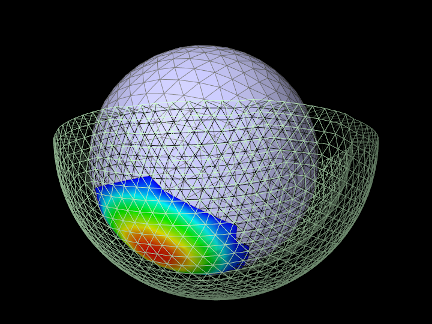
\includegraphics[]{images/ElasticFoundationContact}
\else
 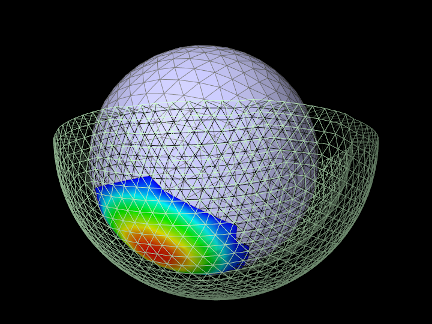
\includegraphics[width=3.75in]{images/ElasticFoundationContact}
\fi
\end{center}
\caption{ElasticFoundationContact showing contact pressure between
the ball and bowl during contact.}
\label{ElasticFoundationContact:fig}
\end{figure}

The source code for the build method is shown below:

\lstset{numbers=left} 
\iflatexml
%% Hack: latexml lstinputlisting doesn't handle firstline correctly
\lstset{firstnumber={-22}}
\lstinputlisting[firstline=1]{../../src/artisynth/demos/tutorial/ElasticFoundationContact.java}
\lstset{firstnumber={1}}
\else
\lstinputlisting[firstline=24]{../../src/artisynth/demos/tutorial/ElasticFoundationContact.java}
\fi
\lstset{numbers=none}

The demo first creates the ball and the bowl as rigid bodies (lines
6-26), with the bowl defined by a mesh read from the file {\tt
data/bowl.obj} relative to the demo source directory, and the ball
defined as an icosahedral sphere. The bowl is fixed in place ({\tt
bowl.setDynamic(false)}), and the ball is positioned at a suitable
location for dropping into the bowl when simulation begins.

Next, a collision behavior is created, with its collision {\sf method}
property set to {\tt VERTEX\_PENETRATION} (as required for EFC), and a
friction coefficient of 0.1 (to ensure that the ball will actually
roll) (lines 28-31). A {\tt LinearElasticContact} is then constructed,
with $E = 10^5$, $\nu=0.4$, damping factor $0.1$, and thickness $0.1$,
and added to the collision behavior using {\tt setForceBehavior()}
(lines 32-26). The behavior is then used to enable contact between the
ball and bowl (line 39).

Lines 41-49 set up rendering properties: the collision manager is made
visible, with color map rendering set to {\tt CONTACT\_PRESSURE}, and
the ball and bowl are set to be rendered in pale blue and green, with
the bowl rendered using only mesh edges so as to make it transparent.

Finally, a control panel is created allowing the user to adjust
properties of the contact force behavior and the pressure rendering
range (lines 51-57).

To run this example in ArtiSynth, select {\sf All demos > tutorial >
ElasticFoundationContact} from the {\sf Models} menu. Running the
model will cause the ball to drop into the bowl, with the resulting
contact pressures rendered as in
Figure \ref{ElasticFoundationContact:fig}.

\subsection{Example: binding EFC properties to fields}
\label{BindingEFCPropsToFields:sec}

It is possible to bind certain EFC material properties to a field, for
situations where these properties vary over the surface of the
contacting meshes. Properties of 
\javaclass[artisynth.core.materials]{LinearElasticContact}
that can be bound to (scalar) fields include {\sf YoungsModulus} and
{\sf thickness}, using the methods 
%
\begin{lstlisting}[]
  setYoungsModulusField (ScalarFieldComponent fcomp)

  setThicknessField (ScalarFieldComponent fcomp)
\end{lstlisting}
%
Most typically, the properties will be bound to a mesh field
(Section \ref{sec:meshFields}) defined with respect to one of the
colliding meshes.

When determining the value of either {\sf youngsModulus} or {\sf
thickness} within its {\tt computeResponse()} method, \pdfbreak
{\tt LinearElasticContact} checks to see if the property is bound to a
field. If it is, the method first checks if the field is a mesh field
associated with the meshes of either {\tt cpnt0} or {\tt cpnt1}, and
if so, extracts the value using the vertex information of the
associated contact point. Otherwise, the value is extracted from the
field using the position of {\tt cpnt0}.

A simple example of binding the {\sf thickness} property to a field is
given by
%
\begin{verbatim}
  artisynth.demos.tutorial.VariableElasticContact
\end{verbatim}
%
This implements EFC between a beveled cylinder and a plate on which
it is resting. The plate is made transparent, allowing the contact
pressure to be viewed from below.

\begin{figure}[ht]
\begin{center}
\begin{tabular}{cc}
\iflatexml
 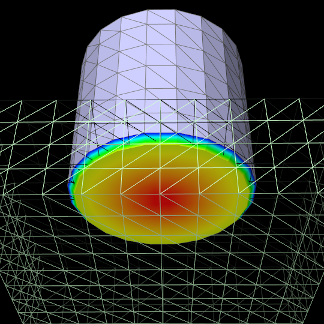
\includegraphics[]{images/VariableElasticContact}
 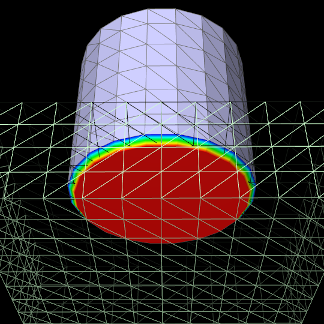
\includegraphics[]{images/VariableElasticContactNF}
\else
 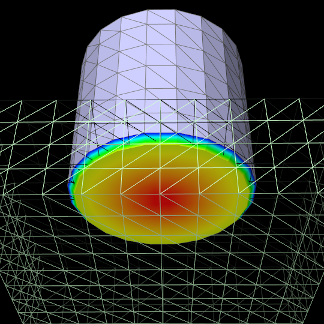
\includegraphics[width=2.8in]{images/VariableElasticContact}
 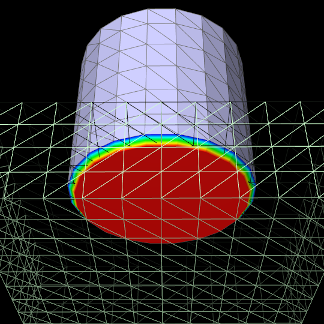
\includegraphics[width=2.8in]{images/VariableElasticContactNF}
\fi
\end{tabular}
\end{center}
\caption {VariableElasticContact showing the contact pressure decreasing
radially from the cylinder center, as the EFC {\sf thickness} property
increases due to its field binding (left). Without the field
binding, the thickness and the pressure are constant across
the cylinder bottom (right).}
\label{VariableElasticContact:fig}
\end{figure}

The model's code is similar to that for {\tt ElasticFoundationContact}
(Section \ref{ElasticFoundationContactDemo:sec}), except that the
collidables are different and the EFC {\sf thickness} property
is bound to a field. The source code for the first part of the build
method is shown below:

\lstset{numbers=left} 
\iflatexml
%% Hack: latexml lstinputlisting doesn't handle firstline correctly
\lstset{firstnumber={-24}}
\lstinputlisting[firstline=1,lastline=53]{../../src/artisynth/demos/tutorial/VariableElasticContact.java}
\lstset{firstnumber={1}}
\else
\lstinputlisting[firstline=26,lastline=78]{../../src/artisynth/demos/tutorial/VariableElasticContact.java}
\fi
\lstset{numbers=none}

First, the cylinder and the plate are created as rigid bodies (lines
6-23), with the cylinder defined by a mesh read from the file {\tt
data/beveledCylinder.obj} relative to the demo source directory.  The
plate is fixed in place and positioned so that it is directly under
the cylinder.

Next, the contact method is set to {\tt VERTEX\_PENETRATION} (as
required for EFC), this time by setting it for all collisions in the
collision manager, and a {\tt LinearElasticContact} is constructed,
with $E = 10^5$, $\nu=0.4$, damping factor $0.1$, and thickness $0.1$
(lines 25-32). Then in lines 34-43, a {\tt ScalarMeshField} is created
for the cylinder surface mesh, with vertex values set so that the
field defines a thickness value $h$ that increases with the radial
distance $r$ from the cylinder axis according to:
%
\begin{equation*}
h = \text{thickness}\; (1+r)
\end{equation*}
%
This field is then added to the {\tt fields} list of the {\tt
MechModel} and the EFC {\sf thickness} property is bound to it
(lines 44-46).

Lastly, a collision behavior is created, with the EFC added to it as a
force behavior, and used to enable cylinder/plate collisions (lines
48-53).

\begin{sideblock}
It is important that EFC properties are bound to fields {\it before}
the behavior method {\tt setForceBehavior()} is called, because that
method {\it copies} the force behavior and so subsequent field
bindings would not be noticed. If for some reason the bindings must be
made after the call, they should be applied to the copied force
behavior, which can be obtained using {\tt getForceBehavior()}.
\end{sideblock}

To run this example in ArtiSynth, select {\sf All demos > tutorial >
VariableElasticContact} from the {\sf Models} menu. Running the model
will result in contact pressures seen in the left of
Figure \ref{VariableElasticContact:fig}, with the pressures decreasing
radially in response to the increasing thickness. With no field
binding, the pressures are constant across the cylinder bottom
(Figure \ref{VariableElasticContact:fig}, right).

\section{Monitoring collisions}
\label{MonitoringCollisions:sec}

Sometimes, an application may wish to know details about the collision
interactions between a specific collidable and one or more other
collidables.  These details may include items such as contact forces
or the penetration regions between the opposing meshes.  This section
describes ways in which these details can be observed through the use
of {\it collision responses}.

\subsection{Collision responses}
\label{collisionResponse:sec}

Applications can track collision information by
creating \javaclass[artisynth.core.mechmodels]{CollisionResponse}
components for the collidables in question and adding them to the {\tt
MechModel} using 
\javamethod*[artisynth.core.mechmodels.MechModel]{setCollisionResponse(,,)}:
%
\begin{lstlisting}[]
   CollisionResponse resp = new CollisionResponse();
   mech.setCollisionResponse (collidable0, collidable1, resp);
\end{lstlisting}
%
An alternate version of {\tt setCollisionResponse()} creates the
response component internally and returns it:
%
\begin{lstlisting}[]
   CollisionResponse resp = mech.setCollisionResponse (collidable0, collidable1);
\end{lstlisting}
%
During every simulation step, the {\tt MechModel} will update its
response components to reflect the current collision conditions
between the associated collidables.

The first collidable specified for a collision response
must be a specific collidable component, while the second may be either another
collidable or a group of collidables represented by a
\javaclass[artisynth.core.mechmodels]{Collidable\$Group}:
%
\begin{lstlisting}[]
  CollisionResponse r0, r1, r2;
  RigidBody bodA;
  FemModel3d femB;

  // collision information between bodA and femB only:
  r0 = setCollisionResponse (bodA, femB); 
  // collision information between femB and all rigid bodies:
  r1 = setCollisionResponse (femB, Collidable.Rigid); 
  // collision information between femB and all bodies and self-collisions:
  r2 = setCollisionResponse (femB, Collidable.All); 
\end{lstlisting}
%
When a compound collidable is specified, the response component will
collect collision information for all its subcollidables.

As as with collision behaviors, the same response cannot be added to
an application twice:
%
\begin{lstlisting}[]
   CollisionResponse resp = new CollisionResponse();
   mech.setCollisionResponse (femA, femB, resp);
   mech.setCollisionResponse (femC, femD, resp); // ERROR
\end{lstlisting}
%

The complete set of methods for managing collision responses are
similar to those for behaviors,
%
\begin{lstlisting}[]
   getCollisionResponse (collidable0, collidable1)
   setCollisionResponse (collidable0, collidable1, response)
   setCollisionResponse (collidable0, collidable1)

   clearCollisionResponse (collidable0, collidable1)
   clearCollisionResponses ()
\end{lstlisting}
%
where
\javamethod*[artisynth.core.mechmodels.MechModel]{getCollisionResponse()}
and
\javamethod*[artisynth.core.mechmodels.MechModel]{clearCollisionResponse()}
respectively return and clear response components that have been
previously set using one of the {\tt setCollisionResponse()} methods.

\subsection{Available information}

Information that can be obtained from a
\javaclass[artisynth.core.mechmodels]{CollisionResponse} component
includes whether or not the collidable is in collision, the current
contact points, forces and pressures acting on the vertices of the
colliding meshes, and the
underlying \javaclass[artisynth.core.mechmodels]{CollisionHandler}
objects that maintain the contact constraints between each colliding
mesh. Much of the available information is similar to that which can
be displayed using collision rendering
(Section \ref{ContactRendering:sec}).

The information methods provided by 
\javaclass[artisynth.core.mechmodels]{CollisionResponse}
are listed below. Many take a {\tt cidx} argument to request
information for either the {\it first} or {\it second} collidable,
which refer, respectively, to the collidables specified by the
arguments {\tt collidable0} and {\tt collidable1} in the {\tt
setCollisionResponse()} methods.

\begin{itemize}

\item {\tt boolean inContact()}

Queries if the collidables associated with the response are in
contact.  Note that this may be true even if the method {\tt getContactData()}
returns an empty list; this can occur, for instance, for vertex
penetration contact when the collision meshes intersect in a small
region without any interpenetrating vertices.

\item {\tt List<ContactData> getContactData()}

Returns a list of the most recently computed contacts between the
collidables. Each contact is described by a {\tt
ContactData} object supplying information about the contact
points on each collidable, the normal, and contact and friction
forces.  If there are no current contacts, the returned list is empty.
For more details on this information, consult the API documentation
for
\javaclass[artisynth.core.mechmodels]{ContactData} and
\javaclass[artisynth.core.modelbase]{ContactPoint}.

\item {\tt Map<Vertex3d,Vector3d> getContactForces(int cidx)}

Returns a map of the contact forces acting the on the vertices of the
collision meshes of either the first or second collidable, as
specified by setting {\tt cidx} to 0 or 1. This information is most
useful and accurate when using vertex penetration contact
(Section \ref{VertexPenetration:sec}).

\item {\tt Map<Vertex3d,Vector3d> getContactForces(int cidx)}

Returns a map of the contact pressures acting the on the vertices of
the collision meshes of either the first or second collidable, as
specified by setting {\tt cidx} to 0 or 1.  This information is most
useful and accurate when using vertex penetration contact
(Section \ref{VertexPenetration:sec}).

\item {\tt ArrayList<PenetrationRegion> getPenetrationRegions(int cidx)}

Returns a list of all the penetration regions on either the first or
second collidable, as specified by setting {\tt cidx} to 0 or
1. Penetration regions are available only if the collision manager's
collider type is set to {\tt AJL\_CONTOUR}
(Section \ref{ColliderTypes:sec}).

\item {\tt ArrayList<CollisionHandler> getHandlers()}

Returns the 
\javaclass[artisynth.core.mechmodels]{CollisionHandler}s
for all currently active collisions associated with the collidables of
the response.

\end{itemize}

A typical usage scenario for collision responses is to create them
before the simulation is run, possibly in the root model {\tt build()}
method, and then query them when the simulation is running, such from
the {\tt apply()} method of a 
\javaclass[artisynth.core.modelbase]{Monitor}
(Section \ref{ControllersAndMonitors:sec}). For example,
in the root model {\tt build()} method, the response
could be created with the call
%
\begin{lstlisting}[]
   CollisionResponse resp = mech.setCollisionResponse (femA, femB);
\end{lstlisting}
%
and then used in some runtime code as follows:
%
\begin{lstlisting}[]
   Map<Vertex3d,Vector3d> collMap = resp.getContactForces (0);
\end{lstlisting}
%
If for some reason it is difficult to store a reference to the
response between its construction and its use, then\pdfbreak
{\tt getCollisionResponse()} can be used to retrieve it:
%
\begin{lstlisting}[]
   CollisionResponse resp = mech.getCollisionResponse (femA, femB);
   Map<Vertex3d,Vector3d> collMap = resp.getContactForces (0);
\end{lstlisting}
%

\begin{sideblock}
As with contact rendering, the information returned by a collision
response may sometimes appear to lag the simulation by one time
step. That is because contacts are computed at the {\it end} of each
time step $i$, and then used to compute the contact forces during the
next step $i+1$. The information returned by a response at the end of
step $i$ is thus based on contacts detected at the end of step $i-1$,
along with contact forces that are computed during step $i$ and used
to calculate the updated positions and velocities at the end of that
step.
\end{sideblock}

\subsection{Example: monitoring contact forces}

\begin{figure}[ht]
\begin{center}
\iflatexml
 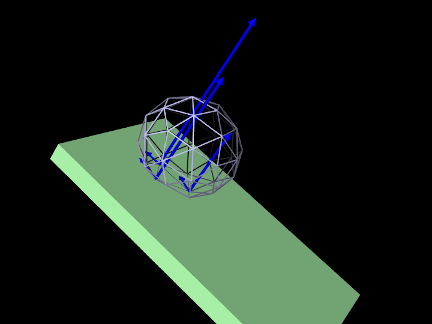
\includegraphics[]{images/ContactForceMonitor}
\else
 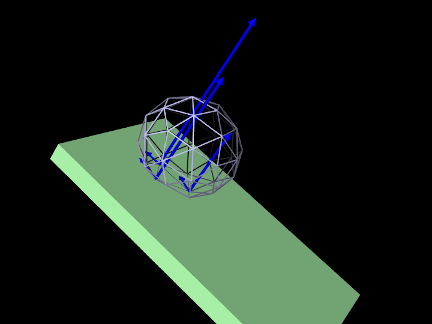
\includegraphics[width=3.6in]{images/ContactForceMonitor}
\fi
\end{center}
\caption {ContactForceMonitor showing the contact forces as
the ball collides with the plane.}
\label{ContactForceMonitor:fig}
\end{figure}

A simple example of using a {\tt CollisionResponse} is given by
%
\begin{verbatim}
  artisynth.demos.tutorial.ContactForceDemo
\end{verbatim}
%
This shows an FEM model of a ball rolling down an inclined plane,
with a collision response combined with a 
\javaclass[artisynth.core.modelbase]{Monitor}
used to print out the contact positions and forces at each time step.
Contact forces are also rendered in the viewer.  The model's source
code, excluding {\tt include} statements, is shown below:

\lstset{numbers=left} 
\iflatexml
%% Hack: latexml lstinputlisting doesn't handle firstline correctly
\lstset{firstnumber={-18}}
\lstinputlisting[firstline=1]{../../src/artisynth/demos/tutorial/ContactForceMonitor.java}
\lstset{firstnumber={1}}
\else
\lstinputlisting[firstline=20]{../../src/artisynth/demos/tutorial/ContactForceMonitor.java}
\fi
\lstset{numbers=none}

The build method creates a simple FEM ball and inclined plane, and
positions the ball to an appropriate drop position (lines 27-42).  The
collisions are enabled between the ball and the plate, along
with a 
\javaclass[artisynth.core.mechmodels]{CollisionResponse}
that is stored in the global reference {\tt myResp} to allow it to be
accessed from the monitor (lines 47-48). 

The monitor itself is implemented by the class {\tt ContactMonitor},
which is created by subclassing
\javaclass[artisynth.core.modelbase]{MonitorBase}
and overriding the {\tt apply()} method to print out the contact
information (lines 5-21). It does this by using the response's {\tt
getContactData()} method to obtain a list of the contacts, and if
there are any, printing the number of contacts, the time step start
time ({\tt t0}), and the position and force of each contact.  An
instance of the monitor is created and added to the root model at line
51.

Rendering is set so that the collision manager renders both the
contact and friction forces in the viewer (lines 55-60), using blue
arrows with a radius of 0.02 (line 60) and a scale factor for the
arrow length of 0.0001 (line 58). To make the ball easy to see
through, its elements are made invisible, and instead is rendered
using only its surface mesh, with face rendering disabled and edges
drawn with a width of 2 (lines 63-67).

To run this example in ArtiSynth, select {\sf All demos > tutorial >
ContactForceMonitor} from the {\sf Models} menu. Running the model
will result in the ball colliding with the plane, showing the contact
and friction forces as blue arrows
(Figure \ref{ContactForceMonitor:fig}, while the monitor prints out
the contact positions and forces to the console at each time step,
producing output like this:
%
\begin{lstlisting}[]
  num contacts: 2, time=0.64
   pos:     -0.918    0.059    0.821, force:  17508.5      0.0  24098.4
   pos:     -0.760   -0.285    0.706, force:  11607.9      0.0  15976.9
  num contacts: 2, time=0.65
   pos:     -0.918    0.059    0.821, force:  16989.6      0.0  23384.2
   pos:     -0.760   -0.285    0.706, force:  11955.8      0.0  16455.7
  num contacts: 3, time=0.66
   pos:     -0.918    0.059    0.821, force:  16465.4      0.0  22662.7
   pos:     -0.760   -0.285    0.706, force:  11880.9      0.0  16352.7
   pos:     -0.695    0.404    0.659, force:    661.1      0.0    910.0
\end{lstlisting}
%


\section{Tips and limitations}
\label{ContactLimitations:sec}

This section describes practical tips that can employed when using
ArtiSynth's contact simulation, together with some of its limitations.

\subsection{Contact jitter}

ArtiSynth's attempt to resolve the interpenetration of colliding
bodies may sometimes cause a jittering behavior around the colliding
area, as the surface collides, separates, and re-collides.  This can
usually be stabilized by maintaining a certain interpenetration
distance during contact. This distance is controlled by the {\tt
MechModel} property {\tt penetrationTol}.  ArtiSynth attempts to
compute a suitable default value for this property, but for some
applications it may be necessary to control the value explicitly using
the {\tt MechModel} methods
%
\begin{lstlisting}[]
   setPenetrationTol (double dist)

   double getPenetrationTol()
\end{lstlisting}
%
\subsection{Passing through objects}
\label{PassingThroughObjects:sec}

The ArtiSynth collision detection mechanism is {\it static}, which
means that mesh intersections are computed at a fixed point in time
and do not presently utilize velocity information. This means that if
the colliding objects are fast enough or thin enough, it is possible
for them to pass completely through each other during a simulation
step (Figure
\ref{passingThroughObjects:fig}, left). Similarly, even if objects
do not pass completely through each other, the penetration may be
large enough for contacts to be established with the wrong side
(\ref{passingThroughObjects:fig}, right).

\begin{figure}[ht]
\begin{center}
\iflatexml
 \includegraphics[]{images/passingThroughObjects}
\else
 \includegraphics[width=3.75in]{images/passingThroughObjects}
\fi
\end{center}
\caption{If object speeds are high enough or the objects thin enough, it
is possible for collidables to pass completely through each other
(left), or to penetrate sufficiently that contacts are established
with the wrong side (right).}
\label{passingThroughObjects:fig}
\end{figure}

When this happens, there are two straightforward solutions:

\begin{enumerate}

\item Reduce the simulation step size.

\item Increase the thickness of one or more of the colliding meshes.
This option is facilitated by the fact that, as mentioned in Section
\ref{CollisionMeshesAndCompounds:sec}, collision meshes can be independent
of a collidable's physical geometry.

\end{enumerate}

\begin{sideblock}
The problem of collidables passing through each other can be
particularly acute in the case of shell elements, and consequently
collisions involving shell elements are not fully supported.  However,
collisions involving shell elements will work in some circumstances,
as described in Section \ref{sec:fem:collision}.
\end{sideblock}

\subsection{Stray vertices}

The stray vertex problem sometimes occurs when vertex penetration
contact is used with objects with sharp edges. Because vertex
penetration contacts are determined by finding the nearest face to
each vertex on the opposing mesh, this may sometimes cause an
inappropriate face to be selected if penetration is deep enough and
near a sharp turn in the opposing mesh (Figure
\ref{strayVertices:fig}).

\begin{figure}[ht]
\begin{center}
\iflatexml
 \includegraphics[]{images/strayVertices}
\else
 \includegraphics[width=1.75in]{images/strayVertices}
\fi
\end{center}
\caption{Vertex penetration contact near a sharp turn in the
opposing mesh may sometimes cause the contact to be directed toward
the wrong face, as seen here for the upper left vertex of the
penetrating square.}
\label{strayVertices:fig}
\end{figure}

Possible solutions include:

\begin{enumerate}

\item Reduce the simulation step size.

\item Use the {\tt VERTEX\_EDGE\_PENETRATION} contact method (Section
\ref{SettingContactMethod:sec}).

\item Adjust the mesh geometry or increase the mesh resolution;
higher mesh resolutions will increase the number of contacts
and reduce the impact of stray vertices.

\end{enumerate}

\subsection{Coulomb friction and stability}
\label{FrictionAndStability:sec}

ArtiSynth uses a ``box'' friction approximation
\cite{Lacoursiere07} to compute Coulomb (dry) friction,
which allows for a less expensive and more robust computation at the
expense of some accuracy. Box friction computes friction forces in two
orthogonal directions in the plane perpendicular to the contact
normal, using a fixed normal force taken from the previous solve,
instead of employing the more detailed polyhedralized friction cones
commonly used in multibody dynamics
\cite{AnitescuPotra2002,PotraEtAlTrapezoidal2006}. 
The resulting linear complementarity problem is convex and hence more
easily solved. Errors can be minimized by ensuring that one of the
friction directions is parallel to the tangential contact velocity.

By default, friction forces are computed {\it after} after the main
velocity solve, in a secondary solve that does not use implicit
integration techniques. This reduces compute time and works well for
rigid bodies, or for FEM models when the friction forces are
relatively small (which they often are in biomechanical applications).
However, applications involving FEM models and large friction forces
may suffer from instability. An example of this might be an FEM model
resting on an inclined plane and relying on friction to remain
stationary under a large load. To handle such situations, one can
enable {\it implicit friction integration} by setting the {\sf
useImplicitFriction} property in {\tt MechModel}; this can be done in
code using the {\tt MechModel} methods
%
\begin{lstlisting}[]
   setUseImplicitFriction (boolean enable)

   boolean getUseImplicitFriction()
\end{lstlisting}
%

\begin{sideblock}
At the time of this writing, implicit friction integration is a new
ArtiSynth feature, and should be considered to be in beta testing.

When using implicit friction integration, if redundant contacts arise
(typically between rigid bodies), it may be necessary to regularize
both the contact constraints, using one of the methods described in
Section \ref{ContactRegularization:sec}, as well as the friction
constraints, by setting the {\sf stictionCreep} property of either the
collision manager or behavior to a non-zero value, as described in
Section \ref{CollisionBehavior:sec}.
\end{sideblock}

\ifdefined\maindoc
\else
\end{document}
\fi
